\documentclass[8pt]{beamer}
\usetheme{Madrid}
\usecolortheme{default}
\usepackage{amsmath, amssymb, graphicx, array, multirow, booktabs, xcolor, tikz}
\usetikzlibrary{shapes,arrows,positioning,fit,backgrounds}

% Compact font settings for tutorial format
\setbeamerfont{title}{size=\Large}
\setbeamerfont{subtitle}{size=\small}
\setbeamerfont{author}{size=\scriptsize}
\setbeamerfont{date}{size=\scriptsize}
\setbeamerfont{frametitle}{size=\large}
\setbeamerfont{framesubtitle}{size=\normalsize}
\setbeamerfont{enumerate item}{size=\footnotesize}
\setbeamerfont{itemize item}{size=\footnotesize}
\setbeamerfont{block title}{size=\footnotesize}

% Compact spacing
\setlength{\itemsep}{0.08ex}
\setlength{\parskip}{0.08ex}
\setlength{\leftmargini}{0.3cm}
\setbeamersize{text margin left=3mm, text margin right=3mm}
\addtobeamertemplate{frame begin}{\vspace{-0.4cm}}{}

% Colors for tutorial
\definecolor{blue}{RGB}{0,0,255}
\definecolor{red}{RGB}{255,0,0}
\definecolor{green}{RGB}{0,128,0}
\definecolor{orange}{RGB}{255,165,0}
\definecolor{purple}{RGB}{128,0,128}
\definecolor{gray}{RGB}{128,128,128}
\definecolor{lightblue}{RGB}{173,216,230}
\definecolor{lightyellow}{RGB}{255,255,224}
\definecolor{lightgreen}{RGB}{144,238,144}
\definecolor{lightred}{RGB}{255,182,193}

\title{Reinforcement Learning}
\subtitle{COMPLETE TUTORIAL: MAB, Monte Carlo, TD, DQN, Policy Methods}
\author{GARP RAI Exam Preparation}
\date{}

\begin{document}
	
	\begin{frame}
		\titlepage
	\end{frame}
	
	% ============================================================
	% TUTORIAL INTRODUCTION - SLIDES 1-5
	% ============================================================
	
	\begin{frame}{TUTORIAL OVERVIEW - Reinforcement Learning}
		\fontsize{7}{8}\selectfont
		\textbf{What You Will Learn in This Tutorial:}
		
		\vspace{0.2cm}
		\begin{tabular}{|p{2.5cm}|p{5.5cm}|}
			\hline
			\textcolor{blue}{Topic} & \textcolor{blue}{Key Concepts Covered} \\
			\hline
			1. RL Fundamentals & Agent, Environment, State, Action, Reward, Policy, Value Functions \\
			\hline
			2. Multi-Armed Bandit & Exploration vs Exploitation, $\epsilon$-Greedy, Q-Value Updates \\
			\hline
			3. Monte Carlo Methods & Episode-based Learning, Full Returns, Bias-Variance Trade-off \\
			\hline
			4. Temporal Difference & Online Learning, Bootstrapping, Q-Learning, SARSA, TD Error \\
			\hline
			5. Deep RL \& DQN & Neural Networks, Experience Replay, Target Networks \\
			\hline
			6. Policy Methods & Value-based vs Policy-based, Actor-Critic, Continuous Actions \\
			\hline
		\end{tabular}
		
		\vspace{0.2cm}
		\textbf{Tutorial Format:}
		\begin{itemize}
			\item Each topic presented with \textcolor{blue}{theory}, \textcolor{blue}{mathematics}, \textcolor{blue}{examples}, and \textcolor{blue}{exam traps}
			\item Step-by-step explanations with detailed calculations
			\item Practical tips for risk management applications
		\end{itemize}
		
		\textcolor{red}{\textbf{Key to Success:}} Understand the \textcolor{blue}{"exploration vs exploitation"} trade-off - it is the heart of RL!
	\end{frame}
	
	\begin{frame}{RL - What Makes It Different?}
		\fontsize{6.5}{7.5}\selectfont
		\textcolor{blue}{\textbf{Reinforcement Learning vs Other Paradigms}}
		
		\begin{tabular}{|p{3.5cm}|p{5.5cm}|}
			\hline
			\textcolor{blue}{Paradigm} & \textcolor{blue}{Key Characteristic} \\
			\hline
			Supervised Learning & Learns from \textcolor{blue}{labeled data}; output = prediction/classification \\
			\hline
			Unsupervised Learning & Finds \textcolor{blue}{hidden patterns}; output = clusters/structures \\
			\hline
			Reinforcement Learning & Learns through \textcolor{blue}{trial and error}; output = policy/action \\
			\hline
		\end{tabular}
		
		\textbf{Core RL Concept:}
		\begin{itemize}
			\item Agent \textcolor{blue}{interacts} with environment
			\item Takes \textcolor{blue}{actions}
			\item Receives \textcolor{blue}{rewards} (positive or negative)
			\item Goal: \textcolor{blue}{Maximize cumulative future reward}
		\end{itemize}
		
		\textbf{Analogy - Dog Training:}
		\begin{itemize}
			\item Command $\rightarrow$ Dog takes action $\rightarrow$ Reward if correct
			\item Over time, dog learns the \textcolor{blue}{policy}: command $\rightarrow$ correct action
		\end{itemize}
		
		\textcolor{red}{\textbf{Exam Trap:}} RL is NOT supervised learning - it uses \textcolor{blue}{rewards} as feedback, not labels!
	\end{frame}
	
	\begin{frame}{RL - Key Terminology}
		\fontsize{6.5}{7.5}\selectfont
		\textcolor{blue}{\textbf{The Language of Reinforcement Learning}}
		
		\begin{tabular}{|p{2.5cm}|p{5.5cm}|}
			\hline
			\textcolor{blue}{Term} & \textcolor{blue}{Definition} \\
			\hline
			Agent & The \textcolor{blue}{learner/decision-maker} who takes actions \\
			\hline
			Environment & The \textcolor{blue}{world} the agent interacts with \\
			\hline
			Action (a) & A \textcolor{blue}{choice} the agent can make \\
			\hline
			State (s) & The \textcolor{blue}{current situation} of the environment \\
			\hline
			Reward (R) & \textcolor{blue}{Feedback} from environment (positive or negative) \\
			\hline
			Policy ($\pi$) & The agent's \textcolor{blue}{strategy} - maps states to actions \\
			\hline
			Value Function V(s) & How \textcolor{blue}{good} it is to be in state s \\
			\hline
			Action-Value Q(s,a) & How \textcolor{blue}{good} it is to take action a in state s \\
			\hline
		\end{tabular}
		
		\textbf{Key Insight:}
		\begin{itemize}
			\item The goal is to find the \textcolor{blue}{optimal policy} $\pi^*$ that maximizes reward
			\item If you know Q(s,a) for all actions, the optimal policy is: $\pi^*(s) = \arg\max_a Q(s,a)$
		\end{itemize}
		
		\textcolor{red}{\textbf{Exam Trap:}} Policy $\neq$ Value Function. Policy is the \textcolor{blue}{strategy}; Value Function is the \textcolor{blue}{estimate of goodness}!
	\end{frame}
	
	\begin{frame}{RL - Mathematical Framework}
		\fontsize{6.5}{7.5}\selectfont
		\textcolor{blue}{\textbf{The Mathematics of Reinforcement Learning}}
		
		\textbf{Expected Future Return (G):}
		\[
		G_t = R_{t+1} + \gamma R_{t+2} + \gamma^2 R_{t+3} + \cdots
		\]
		where $\gamma$ is the \textcolor{blue}{discount factor} ($0 \leq \gamma \leq 1$)
		
		\textbf{State-Value Function V(s):}
		\[
		V_\pi(s) = E_\pi[G_t | S_t = s]
		\]
		Measures how good it is to be in state s under policy $\pi$
		
		\textbf{Action-Value Function Q(s,a):}
		\[
		Q_\pi(s,a) = E_\pi[G_t | S_t = s, A_t = a]
		\]
		Measures how good it is to take action a in state s
		
		\textbf{Relationship Between V and Q:}
		\[
		V_\pi(s) = \sum_a \pi(a|s) Q_\pi(s,a)
		\]
		\[
		V^*(s) = \max_a Q^*(s,a)
		\]
		
		\textcolor{red}{\textbf{Exam Trap:}} V(s) is the \textcolor{blue}{expectation over actions}; Q(s,a) is \textcolor{blue}{action-specific}!
	\end{frame}
	
	\begin{frame}{RL - Famous Applications}
		\fontsize{6.5}{7.5}\selectfont
		\textcolor{blue}{\textbf{Real-World RL Applications}}
		
		\textbf{AlphaGo / AlphaZero (DeepMind):}
		\begin{itemize}
			\item Learned to play Go, Chess, Shogi at \textcolor{blue}{superhuman level}
			\item Played \textcolor{blue}{millions} of games against itself
			\item Discovered \textcolor{blue}{novel strategies} humans hadn't found
		\end{itemize}
		
		\textbf{Robotics:}
		\begin{itemize}
			\item Training robots for \textcolor{blue}{complex manipulation}
			\item Self-driving cars
			\item Warehouse automation
		\end{itemize}
		
		\textbf{Business Applications:}
		\begin{itemize}
			\item \textcolor{blue}{Dynamic Pricing}: Adjust prices based on demand
			\item \textcolor{blue}{Supply Chain}: Inventory and routing optimization
			\item \textcolor{blue}{Trading}: Optimal execution of trades
			\item \textcolor{blue}{Chatbots}: RLHF for ChatGPT and other LLMs
		\end{itemize}
		
		\textbf{RLHF - Reinforcement Learning from Human Feedback:}
		\begin{itemize}
			\item Humans rank model outputs
			\item RL algorithm adjusts to \textcolor{blue}{maximize human scores}
			\item Key to modern LLM capabilities
		\end{itemize}
		
		\textcolor{red}{\textbf{Exam Trap:}} RLHF is a key technique for \textcolor{blue}{fine-tuning LLMs} - not just for games!
	\end{frame}
	
	% ============================================================
	% SECTION 1: MULTI-ARMED BANDIT - SLIDES 6-25
	% ============================================================
	
	\begin{frame}{MAB - Introduction}
		\fontsize{6.5}{7.5}\selectfont
		\textcolor{blue}{\textbf{The Multi-Armed Bandit Problem}}
		
		\textbf{The Scenario:}
		\begin{itemize}
			\item A gambler (agent) faces \textcolor{blue}{multiple slot machines}
			\item Each machine has \textcolor{blue}{unknown} reward distribution
			\item Goal: \textcolor{blue}{Maximize total winnings} over many plays
		\end{itemize}
		
		\textbf{Key Characteristics of MAB:}
		\begin{enumerate}
			\item \textcolor{blue}{Single state} - environment doesn't change
			\item Actions don't affect future states
			\item Each action gives an \textcolor{blue}{immediate reward}
			\item No long-term consequences of actions
		\end{enumerate}
		
		\textbf{Why MAB Matters:}
		\begin{itemize}
			\item \textcolor{blue}{Foundation} for understanding RL
			\item Introduces the \textcolor{blue}{exploration vs exploitation} dilemma
			\item Real-world applications: A/B testing, ad optimization
		\end{itemize}
		
		\textbf{The Core Dilemma:}
		\begin{itemize}
			\item \textcolor{blue}{Exploit}: Play the machine that has been best so far
			\item \textcolor{blue}{Explore}: Try other machines to find if they are better
			\item Neither pure exploration nor pure exploitation is optimal
		\end{itemize}
		
		\textcolor{red}{\textbf{Exam Trap:}} MAB has \textcolor{blue}{ONLY ONE STATE} - this is what makes it simpler than general RL!
	\end{frame}
	
	\begin{frame}{MAB - The Three Strategies}
		\fontsize{6.5}{7.5}\selectfont
		\textcolor{blue}{\textbf{Three Strategies for MAB}}
		
		\textbf{Strategy 1: Greedy (Pure Exploitation)}
		\begin{itemize}
			\item Always choose the machine with the \textcolor{blue}{highest Q-value}
			\item Pros: Maximizes immediate reward
			\item Cons: May miss a better machine that was never tried
		\end{itemize}
		
		\textbf{Strategy 2: Random (Pure Exploration)}
		\begin{itemize}
			\item Always choose a \textcolor{blue}{random} machine
			\item Pros: Gathers information about all machines
			\item Cons: Never uses information to maximize reward
		\end{itemize}
		
		\textbf{Strategy 3: $\epsilon$-Greedy (Balanced)}
		\begin{itemize}
			\item With probability $\epsilon$: \textcolor{blue}{Explore} (random action)
			\item With probability $1-\epsilon$: \textcolor{blue}{Exploit} (best action so far)
			\item Pros: \textcolor{green}{Balances} exploration and exploitation
			\item Common refinement: \textcolor{blue}{Decay $\epsilon$} over time
		\end{itemize}
		
		\textbf{Visual Decision Process:}
		\begin{center}
			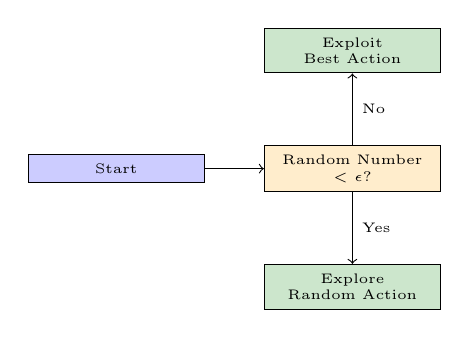
\begin{tikzpicture}[scale=0.5, every node/.style={font=\tiny}]
				\node[draw, rectangle, fill=blue!20, text width=2cm, align=center] (start) {Start};
				\node[draw, rectangle, fill=orange!20, text width=2cm, align=center] (rand) [right of=start, xshift=2cm] {Random Number\\$<$ $\epsilon$?};
				\node[draw, rectangle, fill=green!20, text width=2cm, align=center] (explore) [below of=rand, yshift=-0.5cm] {Explore\\Random Action};
				\node[draw, rectangle, fill=green!20, text width=2cm, align=center] (exploit) [above of=rand, yshift=0.5cm] {Exploit\\Best Action};
				\draw[->] (start) -- (rand);
				\draw[->] (rand) -- (explore) node[midway,right] {Yes};
				\draw[->] (rand) -- (exploit) node[midway,right] {No};
			\end{tikzpicture}
		\end{center}
		
		\textcolor{red}{\textbf{Exam Trap:}} $\epsilon$-greedy with decay is usually the \textcolor{blue}{best practical} strategy!
	\end{frame}
	
	\begin{frame}{MAB - Q-Value Calculation}
		\fontsize{6.5}{7.5}\selectfont
		\textcolor{blue}{\textbf{How Q-Values Are Calculated in MAB}}
		
		\textbf{Q-Value = Average of Observed Rewards:}
		\[
		Q_k^n = \frac{1}{n}\sum_{j=1}^n R_j
		\]
		where $n$ = number of times machine $k$ has been played
		
		\textbf{Example: Machine A played 5 times:}
		\begin{itemize}
			\item Rewards: [1.2, 0.8, 1.5, 0.3, 1.1]
			\item Sum = 1.2 + 0.8 + 1.5 + 0.3 + 1.1 = 4.9
			\item Q(A) = 4.9 / 5 = 0.98
		\end{itemize}
		
		\textbf{Incremental Update Formula:}
		\[
		Q_k^n = Q_k^{n-1} + \frac{1}{n}(R_n - Q_k^{n-1})
		\]
		\textit{This is computationally efficient - just update the average with new data!}
		
		\textbf{Step-by-Step Example:}
		\begin{enumerate}
			\item Initial: Q = 0, n = 0
			\item Play 1: R = 1.2, Q = 0 + (1/1)(1.2 - 0) = 1.2
			\item Play 2: R = 0.8, Q = 1.2 + (1/2)(0.8 - 1.2) = 1.0
			\item Play 3: R = 1.5, Q = 1.0 + (1/3)(1.5 - 1.0) = 1.167
		\end{enumerate}
		
		\textcolor{red}{\textbf{Exam Trap:}} Q-values are \textcolor{blue}{averages}, not sums or maximums! Update using the incremental formula.
	\end{frame}
	
	\begin{frame}{MAB - $\epsilon$ Decay Calculation}
		\fontsize{6.5}{7.5}\selectfont
		\textcolor{blue}{\textbf{How $\epsilon$ Decays Over Time}}
		
		\textbf{Exponential Decay Formula:}
		\[
		\epsilon_t = \beta^{t-1}
		\]
		where:
		\begin{itemize}
			\item $\beta$ = decay factor ($0 < \beta < 1$)
			\item $t$ = trial number
		\end{itemize}
		
		\textbf{Example with $\beta = 0.85$:}
		
		\begin{tabular}{|c|c|c|}
			\hline
			\textbf{Trial (t)} & \textbf{$\epsilon_t = 0.85^{t-1}$} & \textbf{Decision} \\
			\hline
			1 & 0.85$^0$ = 1.00 & Always Explore \\
			\hline
			2 & 0.85$^1$ = 0.85 & 85\% Explore, 15\% Exploit \\
			\hline
			5 & 0.85$^4$ = 0.522 & 52.2\% Explore, 47.8\% Exploit \\
			\hline
			10 & 0.85$^9$ = 0.232 & 23.2\% Explore, 76.8\% Exploit \\
			\hline
			20 & 0.85$^{19}$ = 0.046 & 4.6\% Explore, 95.4\% Exploit \\
			\hline
			50 & 0.85$^{49}$ = 0.0004 & Almost Pure Exploit \\
			\hline
		\end{tabular}
		
		\textbf{Key Insight:}
		\begin{itemize}
			\item High $\epsilon$ early = \textcolor{blue}{More exploration}
			\item Low $\epsilon$ later = \textcolor{blue}{More exploitation}
			\item When $\epsilon$ approaches 0, the agent is \textcolor{blue}{fully exploiting}
		\end{itemize}
		
		\textcolor{red}{\textbf{Exam Trap:}} $\epsilon$ starts at 1 (trial 1) and decays to 0 - formula is $\epsilon_t = \beta^{t-1}$, not $\beta^t$!
	\end{frame}
	
	\begin{frame}{MAB - Worked Example}
		\fontsize{6.5}{7.5}\selectfont
		\textcolor{blue}{\textbf{MAB - Step-by-Step Worked Example}}
		
		\textbf{Setup:}
		\begin{itemize}
			\item 3 slot machines: A, B, C
			\item True means: $\mu_A = 0.8$, $\mu_B = 0.5$, $\mu_C = 0.7$
			\item Decay factor: $\beta = 0.85$
			\item Rewards drawn from Normal($\mu_i$, 1)
		\end{itemize}
		
		\textbf{Trial 1:} $\epsilon = 1.00$ $\rightarrow$ Random number 0.7 $<$ 1.0 $\rightarrow$ Explore
		\begin{itemize}
			\item Choose Machine A, Reward = 1.2
			\item Q(A) = 1.2, Q(B) = 0, Q(C) = 0
		\end{itemize}
		
		\textbf{Trial 2:} $\epsilon = 0.85$ $\rightarrow$ Random number 0.99 $\ge$ 0.85 $\rightarrow$ Exploit
		\begin{itemize}
			\item Best machine: A (Q=1.2)
			\item Play A, Reward = 0.8
			\item Q(A) = (1.2 + 0.8)/2 = 1.0
		\end{itemize}
		
		\textbf{Trial 3:} $\epsilon = 0.7225$ $\rightarrow$ Random number 0.65 $<$ 0.7225 $\rightarrow$ Explore
		\begin{itemize}
			\item Choose Machine B, Reward = 1.7
			\item Q(B) = 1.7
		\end{itemize}
		
		\textbf{Continue for many trials...}
		
		\textbf{After 10 Trials:}
		\begin{tabular}{|c|c|}
			\hline
			\textbf{Machine} & \textbf{Q-Value} \\
			\hline
			A & 0.80 \\
			\hline
			B & 0.50 \\
			\hline
			C & 0.70 \\
			\hline
		\end{tabular}
		
		\textcolor{red}{\textbf{Exam Trap:}} The estimated Q-values may differ from true means due to \textcolor{blue}{sampling error} - more trials = more accurate estimates!
	\end{frame}
	
	\begin{frame}{MAB - Greedy Strategy Example}
		\fontsize{6.5}{7.5}\selectfont
		\textcolor{blue}{\textbf{Greedy Strategy - The Risk of Pure Exploitation}}
		
		\textbf{Scenario:}
		\begin{itemize}
			\item 3 machines with Q-values after 5 plays:
			\begin{itemize}
				\item Q(A) = 1.5 (from 5 lucky plays)
				\item Q(B) = 0.0 (never played)
				\item Q(C) = 0.0 (never played)
			\end{itemize}
			\item True means: $\mu_A = 0.2$, $\mu_B = 2.0$, $\mu_C = 1.8$
		\end{itemize}
		
		\textbf{Greedy Strategy:}
		\begin{itemize}
			\item Always plays Machine A (highest Q-value = 1.5)
			\item Expected reward per play = 0.2
			\item Total reward = $0.2 \times 1000 = 200$
		\end{itemize}
		
		\textbf{Optimal Strategy (if known):}
		\begin{itemize}
			\item Always plays Machine B (true mean = 2.0)
			\item Expected reward per play = 2.0
			\item Total reward = $2.0 \times 1000 = 2000$
		\end{itemize}
		
		\textbf{The Problem:}
		\begin{itemize}
			\item Greedy got \textcolor{red}{stuck} with a suboptimal machine
			\item \textcolor{blue}{Exploration} would have discovered the better machine
			\item This is why we need $\epsilon$-greedy!
		\end{itemize}
		
		\textbf{Regret:}
		\begin{itemize}
			\item Regret = Reward$_{optimal}$ - Reward$_{actual}$
			\item = 2000 - 200 = 1800 (huge loss!)
		\end{itemize}
		
		\textcolor{red}{\textbf{Exam Trap:}} Greedy strategy can be \textcolor{red}{catastrophically suboptimal} if the initially best machine is not the true best!
	\end{frame}
	
	\begin{frame}{MAB - Random Strategy Example}
		\fontsize{6.5}{7.5}\selectfont
		\textcolor{blue}{\textbf{Random Strategy - The Problem of Pure Exploration}}
		
		\textbf{Scenario:}
		\begin{itemize}
			\item 3 machines with true means: $\mu_A = 0.8$, $\mu_B = 0.5$, $\mu_C = 0.7$
			\item 1000 plays
		\end{itemize}
		
		\textbf{Random Strategy:}
		\begin{itemize}
			\item Always picks a machine \textcolor{blue}{uniformly at random}
			\item Expected reward per play = average of all means
			\item = (0.8 + 0.5 + 0.7) / 3 = 0.667
			\item Total reward = $0.667 \times 1000 = 667$
		\end{itemize}
		
		\textbf{Optimal Strategy (if known):}
		\begin{itemize}
			\item Always plays Machine A (highest mean = 0.8)
			\item Total reward = $0.8 \times 1000 = 800$
		\end{itemize}
		
		\textbf{Comparison:}
		\begin{itemize}
			\item Greedy (if lucky): 800
			\item Random: 667 (about 83\% of optimal)
			\item With $\epsilon$-greedy: typically 700-780 (near optimal)
		\end{itemize}
		
		\textbf{The Problem:}
		\begin{itemize}
			\item Random strategy \textcolor{red}{wastes} knowledge
			\item After 1000 plays, the agent knows which machine is best
			\item But continues to play random machines!
		\end{itemize}
		
		\textcolor{red}{\textbf{Exam Trap:}} Random strategy \textcolor{red}{never exploits} - it ignores all information gained!
	\end{frame}
	
	\begin{frame}{MAB - $\epsilon$-Greedy Example}
		\fontsize{6.5}{7.5}\selectfont
		\textcolor{blue}{\textbf{$\epsilon$-Greedy - The Balanced Approach}}
		
		\textbf{Setup:}
		\begin{itemize}
			\item 3 machines, true means: $\mu_A = 0.8$, $\mu_B = 0.5$, $\mu_C = 0.7$
			\item $\epsilon = 0.10$ (constant)
			\item 1000 plays
		\end{itemize}
		
		\textbf{How It Works:}
		\begin{enumerate}
			\item With probability 0.10: \textcolor{blue}{Explore} - pick random machine
			\item With probability 0.90: \textcolor{blue}{Exploit} - pick best machine so far
		\end{enumerate}
		
		\textbf{Expected Behavior:}
		\begin{itemize}
			\item About 90\% of plays: best machine (A) $\rightarrow$ reward ~0.8
			\item About 10\% of plays: random machines $\rightarrow$ average reward ~0.667
			\item Expected reward per play $\approx$ 0.9(0.8) + 0.1(0.667) = 0.787
			\item Total reward $\approx$ 787 (out of possible 800)
		\end{itemize}
		
		\textbf{Comparison Table:}
		
		\begin{tabular}{|p{3cm}|p{3cm}|p{3cm}|}
			\hline
			\textbf{Strategy} & \textbf{Expected Reward} & \textbf{Regret} \\
			\hline
			Optimal & 800 & 0 \\
			\hline
			$\epsilon$-greedy (0.1) & ~787 & ~13 \\
			\hline
			Greedy (if lucky) & 800 & 0 \\
			\hline
			Greedy (if unlucky) & 200 & 600 \\
			\hline
			Random & 667 & 133 \\
			\hline
		\end{tabular}
		
		\textbf{With Decay ($\epsilon$ decreases over time):}
		\begin{itemize}
			\item Early: More exploration to find best machine
			\item Late: More exploitation to maximize reward
			\item Often \textcolor{blue}{outperforms} constant $\epsilon$
		\end{itemize}
		
		\textcolor{red}{\textbf{Exam Trap:}} $\epsilon$-greedy with decay is usually \textcolor{blue}{better} than fixed $\epsilon$!
	\end{frame}
	
	\begin{frame}{MAB - $\epsilon$ Decay Factor Analysis}
		\fontsize{6.5}{7.5}\selectfont
		\textcolor{blue}{\textbf{Choosing the Decay Factor $\beta$}}
		
		\textbf{Effect of Different $\beta$ Values:}
		
		\begin{tabular}{|c|c|c|c|}
			\hline
			\textbf{Trial (t)} & $\beta = 0.85$ & $\beta = 0.95$ & $\beta = 0.99$ \\
			\hline
			1 & 1.00 & 1.00 & 1.00 \\
			\hline
			5 & 0.522 & 0.815 & 0.961 \\
			\hline
			10 & 0.232 & 0.630 & 0.914 \\
			\hline
			20 & 0.046 & 0.377 & 0.827 \\
			\hline
			50 & 0.0004 & 0.077 & 0.606 \\
			\hline
			100 & $\approx$0 & 0.006 & 0.366 \\
			\hline
			200 & $\approx$0 & $3\times10^{-5}$ & 0.134 \\
			\hline
		\end{tabular}
		
		\textbf{Interpretation:}
		\begin{itemize}
			\item $\beta = 0.85$: \textcolor{blue}{Fast decay} - explores early, exploits quickly
			\begin{itemize}
				\item Good for simple problems where best action is found quickly
			\end{itemize}
			\item $\beta = 0.95$: \textcolor{blue}{Moderate decay} - balanced approach
			\begin{itemize}
				\item Good for most practical problems
			\end{itemize}
			\item $\beta = 0.99$: \textcolor{blue}{Slow decay} - explores for a long time
			\begin{itemize}
				\item Good for complex problems where best action is hard to find
			\end{itemize}
		\end{itemize}
		
		\textbf{When $\epsilon$ Becomes Very Small:}
		\begin{itemize}
			\item After ~57 trials with $\beta=0.85$: $\epsilon \approx 0$
			\item After ~230 trials with $\beta=0.95$: $\epsilon \approx 0$
			\item After ~2300 trials with $\beta=0.99$: $\epsilon \approx 0$
		\end{itemize}
		
		\textcolor{red}{\textbf{Exam Trap:}} Smaller $\beta$ = faster decay = \textcolor{blue}{less exploration later}!
	\end{frame}
	
	\begin{frame}{MAB - Thompson Sampling}
		\fontsize{6.5}{7.5}\selectfont
		\textcolor{blue}{\textbf{Thompson Sampling - A Bayesian Alternative}}
		
		\textbf{The Concept:}
		\begin{itemize}
			\item Instead of fixed $\epsilon$, maintain a \textcolor{blue}{probability distribution} for each machine
			\item Sample from each distribution and choose the \textcolor{blue}{maximum sampled value}
			\item Naturally balances exploration and exploitation
		\end{itemize}
		
		\textbf{How It Works:}
		\begin{enumerate}
			\item Each machine has a Beta distribution (for binary rewards) or Normal distribution (for continuous)
			\item Parameters update with each observation (Bayesian updating)
			\item Each trial:
			\begin{enumerate}
				\item Sample a value from each machine's distribution
				\item Choose the machine with the highest sampled value
				\item Observe reward and update distribution
			\end{enumerate}
		\end{enumerate}
		
		\textbf{Example - Binary Rewards (Win/Lose):}
		\begin{itemize}
			\item Machine A: Beta(5, 2) $\rightarrow$ mean = 5/7 = 0.714
			\item Machine B: Beta(2, 3) $\rightarrow$ mean = 2/5 = 0.400
			\item Machine C: Beta(3, 2) $\rightarrow$ mean = 3/5 = 0.600
			\item Sample: A=0.72, B=0.35, C=0.68 $\rightarrow$ Choose A
		\end{itemize}
		
		\textbf{Advantages over $\epsilon$-Greedy:}
		\begin{itemize}
			\item No $\epsilon$ parameter to tune
			\item Naturally balances exploration based on uncertainty
			\item Machines with high uncertainty get explored more
			\item Theoretically optimal (Bayesian)
		\end{itemize}
		
		\textbf{Disadvantages:}
		\begin{itemize}
			\item Requires assumptions about reward distribution
			\item More computationally expensive
		\end{itemize}
		
		\textcolor{red}{\textbf{Exam Trap:}} Thompson Sampling is \textcolor{blue}{Bayesian} - it maintains uncertainty and samples from it!
	\end{frame}
	
	\begin{frame}{MAB - Regret Analysis}
		\fontsize{6.5}{7.5}\selectfont
		\textcolor{blue}{\textbf{Regret - Measuring Performance in MAB}}
		
		\textbf{Definition:}
		\[
		\text{Regret}(T) = T \times \mu^* - \sum_{t=1}^T \mu_{a_t}
		\]
		where:
		\begin{itemize}
			\item $T$ = total number of trials
			\item $\mu^*$ = true mean of the best machine
			\item $\mu_{a_t}$ = true mean of the machine played at time $t$
		\end{itemize}
		
		\textbf{Interpretation:}
		\begin{itemize}
			\item Regret is the \textcolor{blue}{opportunity cost} of not knowing the best machine
			\item Cumulative loss from suboptimal choices
			\item Goal of RL: \textcolor{blue}{Minimize regret}
		\end{itemize}
		
		\textbf{Example:}
		\begin{itemize}
			\item True means: $\mu_A = 0.8$, $\mu_B = 0.5$, $\mu_C = 0.7$
			\item $\mu^* = 0.8$ (Machine A)
			\item If agent plays Machine B 100 times:
			\begin{itemize}
				\item Regret per play = 0.8 - 0.5 = 0.3
				\item Total regret = 0.3 $\times$ 100 = 30
			\end{itemize}
		\end{itemize}
		
		\textbf{Expected Regret for Different Strategies:}
		
		\begin{tabular}{|p{3cm}|p{3cm}|}
			\hline
			\textbf{Strategy} & \textbf{Expected Regret (T=1000)} \\
			\hline
			Optimal & 0 \\
			\hline
			$\epsilon$-greedy (0.1) & ~13 \\
			\hline
			Greedy (unlucky) & ~600 \\
			\hline
			Random & ~133 \\
			\hline
		\end{tabular}
		
		\textbf{Key Insight:}
		\begin{itemize}
			\item Good algorithms achieve \textcolor{blue}{sublinear regret} - grows slower than T
			\item $\epsilon$-greedy with decay achieves $O(\log T)$ regret
			\item This means average regret per trial $\rightarrow$ 0 as T $\rightarrow \infty$
		\end{itemize}
		
		\textcolor{red}{\textbf{Exam Trap:}} Regret is \textcolor{blue}{cumulative loss} from suboptimal choices - minimize it!
	\end{frame}
	
	\begin{frame}{MAB - Real-World Application: A/B Testing}
		\fontsize{6.5}{7.5}\selectfont
		\textcolor{blue}{\textbf{A/B Testing as a Multi-Armed Bandit Problem}}
		
		\textbf{Traditional A/B Testing:}
		\begin{itemize}
			\item Split traffic 50/50 between options
			\item Test for statistical significance
			\item Then implement the winner
			\item Problem: \textcolor{red}{Wastes traffic} on inferior options
		\end{itemize}
		
		\textbf{MAB Approach to A/B Testing:}
		\begin{itemize}
			\item Treat each variant as a \textcolor{blue}{slot machine}
			\item Use $\epsilon$-greedy or Thompson Sampling
			\item Dynamically allocate more traffic to better-performing variants
			\item Gradually learn which variant is best
		\end{itemize}
		
		\textbf{Example - Ad Click-Through Rates:}
		\begin{itemize}
			\item Variant A: 5\% CTR (true)
			\item Variant B: 3\% CTR (true)
			\item Variant C: 4\% CTR (true)
		\end{itemize}
		
		\textbf{Traditional A/B Test (100,000 impressions):}
		\begin{itemize}
			\item Each variant gets 33,333 impressions
			\item Expected clicks = 0.05(33,333) + 0.03(33,333) + 0.04(33,333) = 4,000
		\end{itemize}
		
		\textbf{MAB Approach (100,000 impressions):}
		\begin{itemize}
			\item Early: Explore all variants
			\item Later: Allocate ~90\% to best variant (A)
			\item Expected clicks $\approx$ 0.9(0.05)(100,000) + 0.05(0.03)(100,000) + 0.05(0.04)(100,000)
			\item $\approx$ 4,500 + 150 + 200 = 4,850
			\item \textcolor{green}{21\% more clicks than A/B test!}
		\end{itemize}
		
		\textcolor{red}{\textbf{Exam Trap:}} MAB can significantly \textcolor{blue}{outperform} traditional A/B testing by reducing regret!
	\end{frame}
	
	\begin{frame}{MAB - Summary and Key Takeaways}
		\fontsize{6.5}{7.5}\selectfont
		\textcolor{blue}{\textbf{MAB - Complete Summary}}
		
		\textbf{Key Concepts to Remember:}
		
		\begin{enumerate}
			\item \textcolor{blue}{MAB Characteristics:}
			\begin{itemize}
				\item Single state (environment doesn't change)
				\item Actions give immediate rewards
				\item No long-term consequences
			\end{itemize}
			
			\item \textcolor{blue}{Three Strategies:}
			\begin{enumerate}
				\item Greedy = Pure exploitation (risks missing better options)
				\item Random = Pure exploration (ignores learned knowledge)
				\item $\epsilon$-Greedy = Balanced approach (best practical choice)
			\end{enumerate}
			
			\item \textcolor{blue}{Q-Value Update:}
			\begin{itemize}
				\item $Q_k^n = \frac{1}{n}\sum R_j$ (average of observed rewards)
				\item Incremental: $Q_k^n = Q_k^{n-1} + \frac{1}{n}(R_n - Q_k^{n-1})$
			\end{itemize}
			
			\item \textcolor{blue}{$\epsilon$ Decay:}
			\begin{itemize}
				\item $\epsilon_t = \beta^{t-1}$
				\item Smaller $\beta$ = faster decay = less exploration later
			\end{itemize}
			
			\item \textcolor{blue}{Regret:}
			\begin{itemize}
				\item Loss from not knowing the optimal action
				\item Goal: Minimize cumulative regret
			\end{itemize}
		\end{enumerate}
		
		\textcolor{red}{\textbf{Exam Success:}} MAB is the foundation of RL - master it and the rest follows!
	\end{frame}
	
	% ============================================================
	% SECTION 2: MONTE CARLO METHODS - SLIDES 26-40
	% ============================================================
	
	\begin{frame}{Monte Carlo - Introduction}
		\fontsize{6.5}{7.5}\selectfont
		\textcolor{blue}{\textbf{Monte Carlo Methods - Learning from Complete Episodes}}
		
		\textbf{What is Monte Carlo RL?}
		\begin{itemize}
			\item Learns from \textcolor{blue}{complete episodes}
			\item Episode = full sequence from start to terminal state
			\item Example: Complete game of chess or Nim
		\end{itemize}
		
		\textbf{Key Characteristic:}
		\begin{itemize}
			\item \textcolor{blue}{Wait until episode ends} to update
			\item Uses \textcolor{blue}{actual returns} ($G_t$), not estimates
			\item \textcolor{green}{Unbiased} - learns from real experience
		\end{itemize}
		
		\textbf{MC vs MAB:}
		\begin{itemize}
			\item MAB: Each trial is independent, one-step
			\item MC: Multiple steps per episode, actions affect future states
		\end{itemize}
		
		\textbf{When to Use MC:}
		\begin{itemize}
			\item Tasks with \textcolor{blue}{defined terminal states} (episodic)
			\item When you want \textcolor{blue}{unbiased} estimates
			\item When episodes are not too long
		\end{itemize}
		
		\textbf{Update Formula:}
		\[
		Q(s,a) \leftarrow Q(s,a) + \alpha(G_t - Q(s,a))
		\]
		where $G_t$ is the total return from time $t$ to episode end
		
		\textcolor{red}{\textbf{Exam Trap:}} MC requires \textcolor{blue}{complete episodes} - cannot be used for continuous tasks!
	\end{frame}
	
	\begin{frame}{Monte Carlo - Episode Definition}
		\fontsize{6.5}{7.5}\selectfont
		\textcolor{blue}{\textbf{What is an Episode in Monte Carlo?}}
		
		\textbf{Definition:}
		\begin{itemize}
			\item A \textcolor{blue}{complete trajectory} from start to terminal state
			\item Sequence: $S_0, A_0, R_1, S_1, A_1, R_2, ..., S_T$
			\item Terminal state $S_T$ ends the episode
		\end{itemize}
		
		\textbf{Examples:}
		\begin{enumerate}
			\item \textcolor{blue}{Game of Nim:} Start with 6 coins $\rightarrow$ coin removal $\rightarrow$ last coin wins
			\item \textcolor{blue}{Chess:} Opening move $\rightarrow$ ... $\rightarrow$ Checkmate
			\item \textcolor{blue}{Board Game:} Start $\rightarrow$ moves $\rightarrow$ Win/Lose
		\end{enumerate}
		
		\textbf{Return Calculation:}
		\[
		G_t = R_{t+1} + \gamma R_{t+2} + \gamma^2 R_{t+3} + \cdots + \gamma^{T-t-1} R_T
		\]
		where $T$ is the terminal time step
		
		\textbf{Example - Nim with 6 coins:}
		\begin{itemize}
			\item Episode length: 2 steps (if Player 1 wins)
			\item Step 1: Pick 3 coins (S=6 $\rightarrow$ S=3)
			\item Step 2: Opponent picks 2 coins (S=3 $\rightarrow$ S=1)
			\item Step 3: Player 1 picks 1 coin (S=1 $\rightarrow$ S=0, Win!)
			\item Terminal state: S=0 (no coins left)
		\end{itemize}
		
		\textbf{Update Only at Episode End:}
		\begin{itemize}
			\item No updates happen within the episode
			\item All state-action pairs encountered are updated at episode end
		\end{itemize}
		
		\textcolor{red}{\textbf{Exam Trap:}} MC updates \textcolor{blue}{only at episode end} - no online learning within episodes!
	\end{frame}
	
	\begin{frame}{Monte Carlo - Return Calculation}
		\fontsize{6.5}{7.5}\selectfont
		\textcolor{blue}{\textbf{Calculating Returns in Monte Carlo}}
		
		\textbf{The Return $G_t$ Formula:}
		\[
		G_t = \sum_{k=0}^{T-t-1} \gamma^k R_{t+k+1}
		\]
		
		\textbf{Example - Nim with $\gamma = 1$:}
		\begin{itemize}
			\item Episode: S=6 $\rightarrow$ S=3 $\rightarrow$ S=1 $\rightarrow$ S=0 (Win)
			\item Rewards: $R_1=0, R_2=0, R_3=1$
			\item For step 1 (t=0): $G_0 = 0 + 0 + 1 = 1$
			\item For step 2 (t=1): $G_1 = 0 + 1 = 1$
			\item For step 3 (t=2): $G_2 = 1$
		\end{itemize}
		
		\textbf{Example - Nim with $\gamma = 0.9$:}
		\begin{itemize}
			\item $G_0 = R_1 + 0.9R_2 + 0.9^2R_3 = 0 + 0 + 0.81 = 0.81$
			\item $G_1 = R_2 + 0.9R_3 = 0 + 0.9 = 0.9$
			\item $G_2 = R_3 = 1$
		\end{itemize}
		
		\textbf{Why Discount Future Rewards?}
		\begin{itemize}
			\item Future rewards are \textcolor{blue}{less certain}
			\item Discounting gives more weight to \textcolor{blue}{immediate rewards}
			\item $\gamma$ close to 0: Short-term focus
			\item $\gamma$ close to 1: Long-term focus
		\end{itemize}
		
		\textbf{MC Update:}
		\[
		Q(s,a) \leftarrow Q(s,a) + \alpha(G_t - Q(s,a))
		\]
		The target is the \textcolor{blue}{actual return} $G_t$
		
		\textcolor{red}{\textbf{Exam Trap:}} MC uses \textcolor{blue}{$G_t$} (actual return) as the target, not estimated future values!
	\end{frame}
	
	\begin{frame}{Monte Carlo - First-Visit vs Every-Visit}
		\fontsize{6.5}{7.5}\selectfont
		\textcolor{blue}{\textbf{First-Visit vs Every-Visit MC}}
		
		\textbf{The Distinction:}
		\begin{itemize}
			\item In an episode, the same state-action pair $(s,a)$ may be visited multiple times
			\item Two ways to handle this:
			\begin{enumerate}
				\item \textcolor{blue}{First-Visit MC}: Only update the first time $(s,a)$ is encountered
				\item \textcolor{blue}{Every-Visit MC}: Update every time $(s,a)$ is encountered
			\end{enumerate}
		\end{itemize}
		
		\textbf{First-Visit MC:}
		\begin{itemize}
			\item Track which $(s,a)$ have been seen in the episode
			\item Only update Q(s,a) the \textcolor{blue}{first time} it occurs
			\item Uses the return from that first occurrence
			\item \textcolor{green}{Unbiased} estimate of Q(s,a)
		\end{itemize}
		
		\textbf{Every-Visit MC:}
		\begin{itemize}
			\item Update Q(s,a) \textcolor{blue}{every time} it occurs
			\item Uses the return from each occurrence
			\item \textcolor{orange}{Slightly biased} but often lower variance
		\end{itemize}
		
		\textbf{Example:}
		\begin{itemize}
			\item Episode: (S1,A1), (S2,A2), (S1,A1), (S3,A3), Terminal
			\item First-visit: Update (S1,A1) only once (using first occurrence)
			\item Every-visit: Update (S1,A1) twice (both occurrences)
		\end{itemize}
		
		\textbf{When to Use Each:}
		\begin{itemize}
			\item First-visit: Theoretical purity, unbiased estimates
			\item Every-visit: More sample-efficient, practical use
		\end{itemize}
		
		\textcolor{red}{\textbf{Exam Trap:}} First-visit MC is \textcolor{blue}{unbiased}; Every-visit MC has \textcolor{orange}{lower variance} but slight bias!
	\end{frame}
	
	\begin{frame}{Monte Carlo - NIM Example Step-by-Step}
		\fontsize{6.5}{7.5}\selectfont
		\textcolor{blue}{\textbf{MC Applied to NIM - Step-by-Step Example}}
		
		\textbf{Setup:}
		\begin{itemize}
			\item 6 coins, remove 1, 2, or 3 coins
			\item $\alpha = 0.05$, $\gamma = 1$
			\item Opponent plays randomly (not optimally)
		\end{itemize}
		
		\textbf{Episode 1:}
		\begin{enumerate}
			\item S=6, A=3 $\rightarrow$ S'=3 (opponent picks 2)
			\item S=1, A=1 $\rightarrow$ S'=0 (Player 1 wins!)
			\item Return: $G = 1$ (win)
		\end{enumerate}
		
		\textbf{MC Updates (Episode End):}
		\begin{itemize}
			\item For (6,3): $Q(6,3) = 0 + 0.05(1 - 0) = 0.05$
			\item For (1,1): $Q(1,1) = 0 + 0.05(1 - 0) = 0.05$
		\end{itemize}
		
		\textbf{Episode 2:}
		\begin{enumerate}
			\item S=6, A=1 $\rightarrow$ S'=5 (opponent picks 1)
			\item S=4, A=3 $\rightarrow$ S'=1 (opponent picks 1)
			\item S=0 (Player 1 loses!)
			\item Return: $G = -1$ (loss)
		\end{enumerate}
		
		\textbf{MC Updates (Episode End):}
		\begin{itemize}
			\item For (6,1): $Q(6,1) = 0 + 0.05(-1 - 0) = -0.05$
			\item For (4,3): $Q(4,3) = 0 + 0.05(-1 - 0) = -0.05$
		\end{itemize}
		
		\textbf{After Many Episodes:}
		\begin{itemize}
			\item Q-values converge to optimal values
			\item Optimal strategy: 6 coins $\rightarrow$ pick 2
		\end{itemize}
		
		\textcolor{red}{\textbf{Exam Trap:}} MC updates \textcolor{blue}{all state-action pairs} in the episode using the same $G$ value!
	\end{frame}
	
	\begin{frame}{Monte Carlo - NIM Q-Table Evolution}
		\fontsize{6.5}{7.5}\selectfont
		\textcolor{blue}{\textbf{MC NIM - Q-Table Evolution Over Episodes}}
		
		\textbf{After Episode 1:}
		\begin{tabular}{|c|c|c|c|c|c|c|}
			\hline
			\textbf{Action} & \textbf{S=1} & \textbf{S=2} & \textbf{S=3} & \textbf{S=4} & \textbf{S=5} & \textbf{S=6} \\
			\hline
			Pick 1 & 0.05 & 0 & 0 & 0 & 0 & 0 \\
			\hline
			Pick 2 & 0 & 0 & 0 & 0 & 0 & 0 \\
			\hline
			Pick 3 & 0 & 0 & 0 & 0 & 0 & 0.05 \\
			\hline
		\end{tabular}
		
		\textbf{After Episode 2:}
		\begin{tabular}{|c|c|c|c|c|c|c|}
			\hline
			\textbf{Action} & \textbf{S=1} & \textbf{S=2} & \textbf{S=3} & \textbf{S=4} & \textbf{S=5} & \textbf{S=6} \\
			\hline
			Pick 1 & 0.05 & 0 & 0 & 0 & 0 & -0.05 \\
			\hline
			Pick 2 & 0 & 0 & 0 & 0 & 0 & 0 \\
			\hline
			Pick 3 & 0 & 0 & 0 & -0.05 & 0 & 0.05 \\
			\hline
		\end{tabular}
		
		\textbf{After Episode 3:}
		\begin{itemize}
			\item Q(6,3): $0.05 + 0.05(1 - 0.05) = 0.0975$
			\item Q(1,1): $0.05 + 0.05(1 - 0.05) = 0.0975$
		\end{itemize}
		
		\textbf{After 1,000,000 Episodes:}
		\begin{tabular}{|c|c|c|c|c|c|c|}
			\hline
			\textbf{Action} & \textbf{S=1} & \textbf{S=2} & \textbf{S=3} & \textbf{S=4} & \textbf{S=5} & \textbf{S=6} \\
			\hline
			Pick 1 & 1 & -1 & -0.071 & 0.380 & 0 & 0.774 \\
			\hline
			Pick 2 & 0 & 1 & -1 & -0.110 & 0 & 1 \\
			\hline
			Pick 3 & 0 & 0 & 1 & -0.858 & 0 & 0.020 \\
			\hline
		\end{tabular}
		
		\textbf{Optimal Strategy:}
		\begin{itemize}
			\item S=6: Pick 2 (Q=1)
			\item S=4: Pick 1 (Q=0.380)
			\item S=3: Pick 3 (Q=1)
			\item S=2: Pick 2 (Q=1)
			\item S=1: Pick 1 (Q=1)
		\end{itemize}
		
		\textcolor{red}{\textbf{Exam Trap:}} Q-values converge to 1 for winning actions, -1 for losing actions!
	\end{frame}
	
	\begin{frame}{Monte Carlo - Advantages and Disadvantages}
		\fontsize{6.5}{7.5}\selectfont
		\textcolor{blue}{\textbf{MC - Pros and Cons}}
		
		\textbf{Advantages:}
		\begin{enumerate}
			\item \textcolor{green}{Unbiased estimates} - uses actual returns, not estimates
			\item \textcolor{green}{Simple to understand and implement}
			\item \textcolor{green}{Works well with long episodes} (uses all information)
			\item \textcolor{green}{No bootstrapping} - no risk of propagating errors
		\end{enumerate}
		
		\textbf{Disadvantages:}
		\begin{enumerate}
			\item \textcolor{red}{High variance} - returns can fluctuate significantly
			\item \textcolor{red}{Requires complete episodes} - cannot handle continuous tasks
			\item \textcolor{red}{Slow learning} - must wait until episode end to update
			\item \textcolor{red}{Inefficient for long episodes} - updates are infrequent
		\end{enumerate}
		
		\textbf{When to Use MC:}
		\begin{itemize}
			\item Tasks with \textcolor{blue}{clear terminal states} (episodic)
			\item When you can run many episodes
			\item When you want \textcolor{blue}{unbiased} value estimates
			\item When episode lengths are reasonable
		\end{itemize}
		
		\textbf{Comparison to TD:}
		\begin{tabular}{|p{4cm}|p{4cm}|}
			\hline
			\textcolor{blue}{MC} & \textcolor{blue}{TD} \\
			\hline
			Unbiased & Biased (bootstrapping) \\
			\hline
			High variance & Low variance \\
			\hline
			Episode-end updates & Step-by-step updates \\
			\hline
			Episodic tasks only & Episodic and continuous tasks \\
			\hline
		\end{tabular}
		
		\textcolor{red}{\textbf{Exam Trap:}} MC = \textcolor{blue}{unbiased but high variance}; TD = \textcolor{blue}{biased but low variance}!
	\end{frame}
	
	\begin{frame}{Monte Carlo - Summary}
		\fontsize{6.5}{7.5}\selectfont
		\textcolor{blue}{\textbf{Monte Carlo - Complete Summary}}
		
		\textbf{Key Concepts to Remember:}
		
		\begin{enumerate}
			\item \textcolor{blue}{Definition:}
			\begin{itemize}
				\item Learns from \textcolor{blue}{complete episodes}
				\item Updates only at episode end
				\item Uses actual returns ($G_t$)
			\end{itemize}
			
			\item \textcolor{blue}{Update Formula:}
			\[
			Q(s,a) \leftarrow Q(s,a) + \alpha(G_t - Q(s,a))
			\]
			
			\item \textcolor{blue}{Return Calculation:}
			\[
			G_t = R_{t+1} + \gamma R_{t+2} + \gamma^2 R_{t+3} + \cdots
			\]
			
			\item \textcolor{blue}{First-Visit vs Every-Visit:}
			\begin{itemize}
				\item First-visit: Update only first occurrence (unbiased)
				\item Every-visit: Update all occurrences (lower variance)
			\end{itemize}
			
			\item \textcolor{blue}{Requirements:}
			\begin{itemize}
				\item \textcolor{red}{Must have} terminal states (episodic tasks)
				\item Cannot handle continuous tasks
			\end{itemize}
			
			\item \textcolor{blue}{Trade-off:}
			\begin{itemize}
				\item \textcolor{green}{Unbiased} but \textcolor{red}{high variance}
			\end{itemize}
		\end{enumerate}
		
		\textcolor{red}{\textbf{Exam Success:}} Remember MC's key limitation: \textcolor{blue}{episodic tasks only}!
	\end{frame}
	
	% ============================================================
	% SECTION 3: TEMPORAL DIFFERENCE - SLIDES 41-60
	% ============================================================
	
	\begin{frame}{TD - Introduction}
		\fontsize{6.5}{7.5}\selectfont
		\textcolor{blue}{\textbf{Temporal Difference - Learning Step by Step}}
		
		\textbf{What is TD Learning?}
		\begin{itemize}
			\item Learns from \textcolor{blue}{incomplete episodes}
			\item Updates \textcolor{blue}{after each step} (online learning)
			\item Uses \textcolor{blue}{bootstrapping} - estimates of future values
		\end{itemize}
		
		\textbf{Key Characteristic:}
		\begin{itemize}
			\item \textcolor{blue}{Doesn't wait} for episode end
			\item Updates using $R_{t+1} + \gamma V(s')$
			\item \textcolor{orange}{Biased} but \textcolor{green}{lower variance}
		\end{itemize}
		
		\textbf{TD vs MC:}
		\begin{tabular}{|p{4cm}|p{4cm}|}
			\hline
			\textcolor{blue}{MC} & \textcolor{blue}{TD} \\
			\hline
			Episode-end updates & Step-by-step updates \\
			\hline
			Uses $G_t$ (actual return) & Uses $R_{t+1} + \gamma V(s')$ (estimate) \\
			\hline
			Unbiased & Biased (bootstrapping) \\
			\hline
			High variance & Low variance \\
			\hline
			Episodic only & Episodic and continuous \\
			\hline
		\end{tabular}
		
		\textbf{TD Update Formula (Value Function):}
		\[
		V(s) \leftarrow V(s) + \alpha(R_{t+1} + \gamma V(s') - V(s))
		\]
		
		\textbf{TD Error:}
		\[
		\delta = R_{t+1} + \gamma V(s') - V(s)
		\]
		This is the \textcolor{blue}{"surprise"} - the difference between new information and current estimate
		
		\textcolor{red}{\textbf{Exam Trap:}} TD uses \textcolor{blue}{bootstrapping} - it updates using estimates of future values, not actual returns!
	\end{frame}
	
	\begin{frame}{TD - Bootstrapping Explained}
		\fontsize{6.5}{7.5}\selectfont
		\textcolor{blue}{\textbf{Bootstrapping - The Core of TD Learning}}
		
		\textbf{What is Bootstrapping?}
		\begin{itemize}
			\item Using a \textcolor{blue}{current estimate} to update another estimate
			\item "Pulling yourself up by your own bootstraps"
			\item Instead of waiting for the final outcome, use your current best guess
		\end{itemize}
		
		\textbf{MC vs TD Bootstrapping:}
		\begin{itemize}
			\item \textcolor{blue}{MC}: No bootstrapping - uses actual returns
			\item \textcolor{blue}{TD}: Bootstrapping - uses estimates of future values
		\end{itemize}
		
		\textbf{Example - Nim:}
		\begin{itemize}
			\item S=6, take action that leads to S'=1
			\item MC: Wait until episode end to know $G$
			\item TD: Use $V(1)$ (current estimate) plus immediate reward
		\end{itemize}
		
		\textbf{TD Target:}
		\[
		R_{t+1} + \gamma V(s')
		\]
		\begin{itemize}
			\item This is a \textcolor{blue}{better guess} than $V(s)$ alone
			\item It uses immediate reward plus estimate of future
		\end{itemize}
		
		\textbf{Why Bootstrapping Works:}
		\begin{itemize}
			\item Updates can be made \textcolor{blue}{immediately}
			\item Doesn't require complete episodes
			\item Often \textcolor{green}{converges faster} than MC
		\end{itemize}
		
		\textbf{TD Error:}
		\[
		\delta = R_{t+1} + \gamma V(s') - V(s)
		\]
		\begin{itemize}
			\item Positive $\delta$: New information suggests state is better than thought
			\item Negative $\delta$: New information suggests state is worse than thought
			\item Zero $\delta$: New information matches current estimate
		\end{itemize}
		
		\textcolor{red}{\textbf{Exam Trap:}} Bootstrapping introduces \textcolor{orange}{bias} but \textcolor{green}{reduces variance}!
	\end{frame}
	
	\begin{frame}{TD - Q-Learning}
		\fontsize{6.5}{7.5}\selectfont
		\textcolor{blue}{\textbf{Q-Learning - The Most Popular TD Algorithm}}
		
		\textbf{Q-Learning Update Formula:}
		\[
		Q(s,a) \leftarrow Q(s,a) + \alpha(R_{t+1} + \gamma \max_{a'} Q(s',a') - Q(s,a))
		\]
		
		\textbf{Key Features:}
		\begin{enumerate}
			\item \textcolor{blue}{Off-policy}: Learns optimal policy regardless of behavior policy
			\item \textcolor{blue}{Model-free}: No environment model needed
			\item \textcolor{blue}{TD method}: Uses bootstrapping
		\end{enumerate}
		
		\textbf{Why "Off-Policy"?}
		\begin{itemize}
			\item The update uses $\max_{a'} Q(s',a')$ (the best possible action)
			\item It doesn't matter which action was actually taken
			\item The agent is learning about the \textcolor{blue}{optimal policy}, not the current policy
		\end{itemize}
		
		\textbf{Algorithm Steps:}
		\begin{enumerate}
			\item Initialize Q(s,a) arbitrarily
			\item For each episode:
			\begin{enumerate}
				\item Initialize state s
				\item For each step:
				\begin{enumerate}
					\item Choose a from s using $\epsilon$-greedy (behavior policy)
					\item Take action a, observe R and s'
					\item Update Q(s,a) using TD target
					\item s $\leftarrow$ s'
				\end{enumerate}
			\end{enumerate}
		\end{enumerate}
		
		\textbf{Example - Simple Grid World:}
		\begin{itemize}
			\item State: Position (x,y)
			\item Actions: Up, Down, Left, Right
			\item Reward: +1 at goal, -1 for walls
			\item Q-learning learns optimal path to goal
		\end{itemize}
		
		\textcolor{red}{\textbf{Exam Trap:}} Q-learning is \textcolor{blue}{off-policy} - learns optimal policy while following any policy (usually $\epsilon$-greedy)!
	\end{frame}
	
	\begin{frame}{TD - SARSA}
		\fontsize{6.5}{7.5}\selectfont
		\textcolor{blue}{\textbf{SARSA - On-Policy TD Learning}}
		
		\textbf{SARSA Update Formula:}
		\[
		Q(s,a) \leftarrow Q(s,a) + \alpha(R_{t+1} + \gamma Q(s',a') - Q(s,a))
		\]
		where $a'$ is the \textcolor{blue}{actual action} taken in state $s'$
		
		\textbf{Key Features:}
		\begin{enumerate}
			\item \textcolor{blue}{On-policy}: Learns the policy being followed
			\item \textcolor{blue}{Model-free}: No environment model needed
			\item \textcolor{blue}{TD method}: Uses bootstrapping
		\end{enumerate}
		
		\textbf{Why "On-Policy"?}
		\begin{itemize}
			\item The update uses $Q(s',a')$ where $a'$ is the \textcolor{blue}{actual} next action
			\item The agent learns about the \textcolor{blue}{current policy}, not the optimal policy
			\item Policy and learning are linked
		\end{itemize}
		
		\textbf{SARSA vs Q-Learning:}
		\begin{tabular}{|p{4cm}|p{4cm}|}
			\hline
			\textcolor{blue}{Q-Learning} & \textcolor{blue}{SARSA} \\
			\hline
			Off-policy & On-policy \\
			\hline
			Uses $\max_{a'} Q(s',a')$ & Uses $Q(s',a')$ (actual action) \\
			\hline
			More aggressive & More conservative \\
			\hline
			Learns optimal policy & Learns current policy \\
			\hline
		\end{tabular}
		
		\textbf{SARSA Algorithm Steps:}
		\begin{enumerate}
			\item Initialize Q(s,a) arbitrarily
			\item For each episode:
			\begin{enumerate}
				\item Initialize state s
				\item Choose a from s using policy (e.g., $\epsilon$-greedy)
				\item For each step:
				\begin{enumerate}
					\item Take action a, observe R and s'
					\item Choose a' from s' using policy
					\item Update Q(s,a) using TD target with a'
					\item s $\leftarrow$ s', a $\leftarrow$ a'
				\end{enumerate}
			\end{enumerate}
		\end{enumerate}
		
		\textcolor{red}{\textbf{Exam Trap:}} SARSA is \textcolor{blue}{on-policy}; Q-learning is \textcolor{blue}{off-policy}. SARSA is more conservative!
	\end{frame}
	
	\begin{frame}{TD - Q-Learning vs SARSA Comparison}
		\fontsize{6.5}{7.5}\selectfont
		\textcolor{blue}{\textbf{Q-Learning vs SARSA - Detailed Comparison}}
		
		\textbf{Key Difference:}
		\begin{itemize}
			\item Q-learning: $Q(s,a) \leftarrow Q(s,a) + \alpha(R + \gamma \max_{a'} Q(s',a') - Q(s,a))$
			\item SARSA: $Q(s,a) \leftarrow Q(s,a) + \alpha(R + \gamma Q(s',a') - Q(s,a))$
		\end{itemize}
		
		\textbf{Behavioral Differences:}
		
		\begin{tabular}{|p{4.5cm}|p{4.5cm}|}
			\hline
			\textcolor{blue}{Q-Learning} & \textcolor{blue}{SARSA} \\
			\hline
			Considers the \textcolor{blue}{best possible} next action & Considers the \textcolor{blue}{actual} next action \\
			\hline
			More aggressive - learns risky policies & More conservative - learns safe policies \\
			\hline
			May choose actions that lead to danger if the danger is avoided optimally & May avoid actions that could lead to danger under current policy \\
			\hline
			Learns the \textcolor{blue}{optimal} policy & Learns the \textcolor{blue}{current} policy \\
			\hline
		\end{tabular}
		
		\textbf{Example - Cliff Walking:}
		\begin{itemize}
			\item Agent must walk along a cliff to reach the goal
			\item Falling off cliff gives large negative reward
		\end{itemize}
		
		\textbf{Q-Learning:}
		\begin{itemize}
			\item Learns the optimal path (right next to the cliff)
			\item This path is risky if the agent sometimes makes mistakes
		\end{itemize}
		
		\textbf{SARSA:}
		\begin{itemize}
			\item Learns a safer path (further from the cliff)
			\item Accounts for the fact that the agent may take suboptimal actions
		\end{itemize}
		
		\textbf{Which to Use?}
		\begin{itemize}
			\item Q-learning: When you want optimal policy, can explore safely
			\item SARSA: When safety is important, exploration is risky
		\end{itemize}
		
		\textcolor{red}{\textbf{Exam Trap:}} Q-learning is more \textcolor{blue}{aggressive}; SARSA is more \textcolor{blue}{conservative}!
	\end{frame}
	
	\begin{frame}{TD - NIM Example Step-by-Step}
		\fontsize{6.5}{7.5}\selectfont
		\textcolor{blue}{\textbf{TD Applied to NIM - Step-by-Step Example}}
		
		\textbf{Setup:}
		\begin{itemize}
			\item 6 coins, remove 1, 2, or 3 coins
			\item $\alpha = 0.05$, $\gamma = 1$
			\item Opponent plays randomly
		\end{itemize}
		
		\textbf{Episode 1:}
		\begin{enumerate}
			\item S=6, A=3 $\rightarrow$ S'=3 (opponent picks 2)
			\item S=1, A=1 $\rightarrow$ S'=0 (Player 1 wins!)
		\end{enumerate}
		
		\textbf{TD Updates (Step by Step):}
		\begin{itemize}
			\item \textbf{Step 1:} S=6, A=3, S'=3, R=0
			\begin{itemize}
				\item V(3) = 0 (current estimate, all 0)
				\item TD target = $0 + 1(0) = 0$
				\item Q(6,3) = $0 + 0.05(0 - 0) = 0$
			\end{itemize}
			\item \textbf{Step 2:} S=1, A=1, S'=0, R=1
			\begin{itemize}
				\item V(0) = 0 (terminal state value)
				\item TD target = $1 + 1(0) = 1$
				\item Q(1,1) = $0 + 0.05(1 - 0) = 0.05$
			\end{itemize}
			\item Update V(1): V(1) = max Q(1,a) = 0.05
		\end{itemize}
		
		\textbf{Episode 2:}
		\begin{enumerate}
			\item S=6, A=1 $\rightarrow$ S'=5 (opponent picks 1)
			\item S=4, A=3 $\rightarrow$ S'=1 (opponent picks 1)
			\item S=0 (Player 1 loses!)
		\end{enumerate}
		
		\textbf{TD Updates:}
		\begin{itemize}
			\item \textbf{Step 1:} S=6, A=1, S'=5, R=0
			\begin{itemize}
				\item V(5) = 0
				\item Q(6,1) = 0 + 0.05(0 - 0) = 0
			\end{itemize}
			\item \textbf{Step 2:} S=4, A=3, S'=1, R=0
			\begin{itemize}
				\item V(1) = 0.05 (from Episode 1)
				\item TD target = $0 + 1(0.05) = 0.05$
				\item Q(4,3) = $0 + 0.05(0.05 - 0) = 0.0025$
			\end{itemize}
		\end{itemize}
		
		\textcolor{red}{\textbf{Exam Trap:}} TD updates \textcolor{blue}{within the episode} using V(s') which may already have been updated!
	\end{frame}
	
	\begin{frame}{TD - NIM Q-Table Evolution}
		\fontsize{6.5}{7.5}\selectfont
		\textcolor{blue}{\textbf{TD NIM - Q-Table Evolution Over Episodes}}
		
		\textbf{After Episode 1:}
		\begin{tabular}{|c|c|c|c|c|c|c|}
			\hline
			\textbf{Action} & \textbf{S=1} & \textbf{S=2} & \textbf{S=3} & \textbf{S=4} & \textbf{S=5} & \textbf{S=6} \\
			\hline
			Pick 1 & 0.05 & 0 & 0 & 0 & 0 & 0 \\
			\hline
			Pick 2 & 0 & 0 & 0 & 0 & 0 & 0 \\
			\hline
			Pick 3 & 0 & 0 & 0 & 0 & 0 & 0 \\
			\hline
		\end{tabular}
		V(1) = 0.05
		
		\textbf{After Episode 2:}
		\begin{tabular}{|c|c|c|c|c|c|c|}
			\hline
			\textbf{Action} & \textbf{S=1} & \textbf{S=2} & \textbf{S=3} & \textbf{S=4} & \textbf{S=5} & \textbf{S=6} \\
			\hline
			Pick 1 & 0.05 & 0 & 0 & 0 & 0 & 0 \\
			\hline
			Pick 2 & 0 & 0 & 0 & 0 & 0 & 0 \\
			\hline
			Pick 3 & 0 & 0 & 0 & 0.0025 & 0 & 0 \\
			\hline
		\end{tabular}
		V(1) = 0.05, V(4) = 0.0025
		
		\textbf{After Episode 3:}
		\begin{enumerate}
			\item S=6, A=3, S'=1, R=0
			\begin{itemize}
				\item V(1) = 0.05
				\item Q(6,3) = 0 + 0.05(0.05 - 0) = 0.0025
			\end{itemize}
			\item S=1, A=1, S'=0, R=1
			\begin{itemize}
				\item Q(1,1) = 0.05 + 0.05(1 - 0.05) = 0.0975
			\end{itemize}
		\end{enumerate}
		
		\textbf{After 1,000,000 Episodes:}
		\begin{tabular}{|c|c|c|c|c|c|c|}
			\hline
			\textbf{Action} & \textbf{S=1} & \textbf{S=2} & \textbf{S=3} & \textbf{S=4} & \textbf{S=5} & \textbf{S=6} \\
			\hline
			Pick 1 & 1 & -1 & -0.105 & 0.383 & 0 & 0.845 \\
			\hline
			Pick 2 & 0 & 1 & -1 & 0.058 & 0 & 1 \\
			\hline
			Pick 3 & 0 & 0 & 1 & -0.842 & 0 & 0.011 \\
			\hline
		\end{tabular}
		
		\textbf{Optimal Strategy:} Same as MC - pick 2 when 6 coins remain!
		
		\textcolor{red}{\textbf{Exam Trap:}} Both MC and TD converge to the \textcolor{blue}{same optimal strategy}!
	\end{frame}
	
	\begin{frame}{TD - Advantages and Disadvantages}
		\fontsize{6.5}{7.5}\selectfont
		\textcolor{blue}{\textbf{TD - Pros and Cons}}
		
		\textbf{Advantages:}
		\begin{enumerate}
			\item \textcolor{green}{Can learn online} - updates after each step
			\item \textcolor{green}{Works for continuous tasks} - no terminal state needed
			\item \textcolor{green}{Lower variance} than MC due to bootstrapping
			\item \textcolor{green}{More sample efficient} - uses information immediately
			\item \textcolor{green}{Often converges faster} than MC
		\end{enumerate}
		
		\textbf{Disadvantages:}
		\begin{enumerate}
			\item \textcolor{red}{Biased} - uses estimates of future values
			\item \textcolor{red}{May propagate errors} - initial bad estimates persist
			\item \textcolor{red}{Requires careful tuning} of $\alpha$ and $\gamma$
			\item \textcolor{red}{Can be unstable} with function approximation
		\end{enumerate}
		
		\textbf{When to Use TD:}
		\begin{itemize}
			\item Continuous (non-episodic) tasks
			\item When you need \textcolor{blue}{online learning}
			\item When episodes are very long
			\item When you want \textcolor{blue}{faster learning}
		\end{itemize}
		
		\textbf{Comparison Table:}
		
		\begin{tabular}{|p{4cm}|p{4cm}|}
			\hline
			\textcolor{blue}{MC} & \textcolor{blue}{TD} \\
			\hline
			Unbiased & Biased \\
			\hline
			High variance & Low variance \\
			\hline
			Episode-end updates & Step-by-step updates \\
			\hline
			Episodic tasks only & Episodic and continuous \\
			\hline
			Slower learning & Faster learning \\
			\hline
		\end{tabular}
		
		\textcolor{red}{\textbf{Exam Trap:}} TD is more \textcolor{blue}{flexible} but has \textcolor{orange}{bias}; MC is \textcolor{blue}{unbiased} but less flexible!
	\end{frame}
	
	\begin{frame}{TD - TD($\lambda$) - The Unified View}
		\fontsize{6.5}{7.5}\selectfont
		\textcolor{blue}{\textbf{TD($\lambda$) - Bridging MC and TD}}
		
		\textbf{The Idea:}
		\begin{itemize}
			\item MC = TD(1) - uses full return
			\item TD(0) = One-step TD - uses immediate reward + one lookahead
			\item TD($\lambda$) - combines many n-step returns
		\end{itemize}
		
		\textbf{n-Step Returns:}
		\[
		G_t^{(n)} = R_{t+1} + \gamma R_{t+2} + \cdots + \gamma^{n-1} R_{t+n} + \gamma^n V(s_{t+n})
		\]
		\begin{itemize}
			\item n=1: TD(0) target
			\item n=$\infty$: MC target (when episode ends)
		\end{itemize}
		
		\textbf{$\lambda$-Return:}
		\[
		G_t^\lambda = (1-\lambda)\sum_{n=1}^{\infty} \lambda^{n-1} G_t^{(n)}
		\]
		\begin{itemize}
			\item $\lambda = 0$: TD(0) (one-step)
			\item $\lambda = 1$: MC (full return)
			\item $0 < \lambda < 1$: Mix of n-step returns
		\end{itemize}
		
		\textbf{Intuition:}
		\begin{itemize}
			\item $\lambda$ controls how far into the future you look
			\item Lower $\lambda$: More like TD (lower variance, higher bias)
			\item Higher $\lambda$: More like MC (higher variance, lower bias)
		\end{itemize}
		
		\textbf{TD($\lambda$) Update:}
		\[
		Q(s,a) \leftarrow Q(s,a) + \alpha(G_t^\lambda - Q(s,a))
		\]
		
		\textbf{Advantages:}
		\begin{itemize}
			\item Can be \textcolor{blue}{more efficient} than TD(0)
			\item Can be \textcolor{blue}{more accurate} than MC
			\item Provides a \textcolor{blue}{unified framework}
		\end{itemize}
		
		\textcolor{red}{\textbf{Exam Trap:}} TD($\lambda$) generalizes both MC and TD - $\lambda=0$ = TD, $\lambda=1$ = MC!
	\end{frame}
	
	\begin{frame}{TD - Summary and Key Takeaways}
		\fontsize{6.5}{7.5}\selectfont
		\textcolor{blue}{\textbf{TD - Complete Summary}}
		
		\textbf{Key Concepts to Remember:}
		
		\begin{enumerate}
			\item \textcolor{blue}{TD Learning:}
			\begin{itemize}
				\item Learns \textcolor{blue}{online} - updates after each step
				\item Uses \textcolor{blue}{bootstrapping} - estimates future values
			\end{itemize}
			
			\item \textcolor{blue}{TD Update:}
			\[
			V(s) \leftarrow V(s) + \alpha(R_{t+1} + \gamma V(s') - V(s))
			\]
			
			\item \textcolor{blue}{TD Error:}
			\[
			\delta = R_{t+1} + \gamma V(s') - V(s)
			\]
			
			\item \textcolor{blue}{Q-Learning:}
			\begin{itemize}
				\item Off-policy, uses $\max_{a'} Q(s',a')$
				\item More aggressive
			\end{itemize}
			
			\item \textcolor{blue}{SARSA:}
			\begin{itemize}
				\item On-policy, uses $Q(s',a')$ (actual action)
				\item More conservative
			\end{itemize}
			
			\item \textcolor{blue}{TD($\lambda$):}
			\begin{itemize}
				\item $\lambda=0$ = TD, $\lambda=1$ = MC
				\item Can be more efficient than TD(0)
			\end{itemize}
			
			\item \textcolor{blue}{TD vs MC:}
			\begin{itemize}
				\item TD: Biased, lower variance, online
				\item MC: Unbiased, higher variance, episode-end
			\end{itemize}
		\end{enumerate}
		
		\textcolor{red}{\textbf{Exam Success:}} Understand the \textcolor{blue}{bias-variance trade-off} between MC and TD!
	\end{frame}
	
	% ============================================================
	% SECTION 4: DEEP RL & DQN - SLIDES 61-80
	% ============================================================
	
	\begin{frame}{Deep RL - Introduction}
		\fontsize{6.5}{7.5}\selectfont
		\textcolor{blue}{\textbf{Deep Reinforcement Learning - Scaling RL}}
		
		\textbf{The Problem with Tabular Methods:}
		\begin{itemize}
			\item Q-table stores Q(s,a) for every state-action pair
			\item Number of states can be \textcolor{red}{enormous} (or infinite)
			\item Example: Atari games have $10^{50}$ possible states!
			\item Self-driving cars have continuous state spaces
		\end{itemize}
		
		\textbf{The Solution: Deep RL}
		\begin{itemize}
			\item Use \textcolor{blue}{neural networks} to approximate Q(s,a)
			\item $Q(s,a) \approx Q(s,a; \theta)$ where $\theta$ = network weights
			\item Neural network takes state as input, outputs Q-values for all actions
		\end{itemize}
		
		\textbf{Why Neural Networks?}
		\begin{enumerate}
			\item \textcolor{blue}{Generalization}: Similar states get similar Q-values
			\item \textcolor{blue}{Compact representation}: No need to store all states
			\item \textcolor{blue}{Continuous spaces}: Can handle continuous state inputs
		\end{enumerate}
		
		\textbf{Deep RL Architecture:}
		\begin{center}
			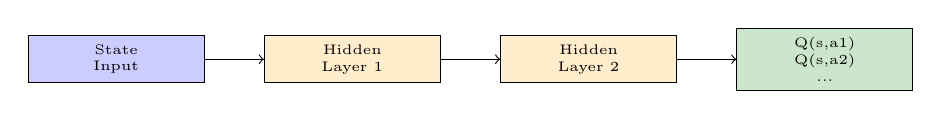
\begin{tikzpicture}[scale=0.5, every node/.style={font=\tiny}]
				\node[draw, rectangle, fill=blue!20, text width=2cm, align=center] (state) {State\\Input};
				\node[draw, rectangle, fill=orange!20, text width=2cm, align=center] (hidden1) [right of=state, xshift=2cm] {Hidden\\Layer 1};
				\node[draw, rectangle, fill=orange!20, text width=2cm, align=center] (hidden2) [right of=hidden1, xshift=2cm] {Hidden\\Layer 2};
				\node[draw, rectangle, fill=green!20, text width=2cm, align=center] (output) [right of=hidden2, xshift=2cm] {Q(s,a1)\\Q(s,a2)\\...};
				\draw[->] (state) -- (hidden1);
				\draw[->] (hidden1) -- (hidden2);
				\draw[->] (hidden2) -- (output);
			\end{tikzpicture}
		\end{center}
		
		\textcolor{red}{\textbf{Exam Trap:}} Deep RL is needed when state spaces are \textcolor{blue}{too large for tables}!
	\end{frame}
	



\begin{frame}{DQN - Introduction}
	\fontsize{6.5}{7.5}\selectfont
	\textcolor{blue}{\textbf{Deep Q-Network - The Breakthrough Algorithm}}
	
	\textbf{What is DQN?}
	\begin{itemize}
		\item Combines Q-learning with \textcolor{blue}{deep neural networks}
		\item Developed by DeepMind (2015)
		\item Achieved human-level performance on Atari games
	\end{itemize}
	
	\textbf{Three Key Innovations:}
	\begin{enumerate}
		\item \textcolor{blue}{Experience Replay}: Store experiences and sample randomly
		\item \textcolor{blue}{Target Network}: Separate network for stable targets
		\item \textcolor{blue}{$\epsilon$-Greedy}: For exploration
	\end{enumerate}
	

\textbf{DQN Architecture:}

\begin{center}
	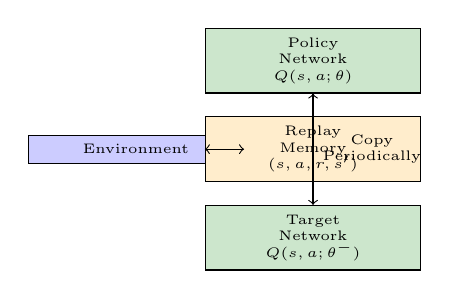
\begin{tikzpicture}[
		scale=0.45,
		every node/.style={font=\tiny}
		]
		
		% Environment
		\node[
		draw,
		rectangle,
		fill=blue!20,
		text width=2.5cm,
		align=center
		] (env) at (0,0) {Environment};
		
		% Replay Memory
		\node[
		draw,
		rectangle,
		fill=orange!20,
		text width=2.5cm,
		align=center
		] (replay) at (5,0) {Replay\\Memory\\$(s,a,r,s')$};
		
		% Policy Network
		\node[
		draw,
		rectangle,
		fill=green!20,
		text width=2.5cm,
		align=center
		] (policy) at (5,2.5) {Policy\\Network\\$Q(s,a;\theta)$};
		
		% Target Network
		\node[
		draw,
		rectangle,
		fill=green!20,
		text width=2.5cm,
		align=center
		] (target) at (5,-2.5) {Target\\Network\\$Q(s,a;\theta^-)$};
		
		% Arrows
		\draw[<->] (env) -- (replay);
		
		\draw[->] (replay) -- (policy);
		
		\draw[->] (policy) -- (target)
		node[midway,right,align=center] {Copy\\Periodically};
		
	\end{tikzpicture}
\end{center}

	
	\textbf{How DQN Works:}
	\begin{enumerate}
		\item Interact with environment and store experiences
		\item Sample a random mini-batch from replay memory
		\item Update the policy network using the TD target from the target network
		\item Periodically copy policy network weights to the target network
	\end{enumerate}
	
	\textcolor{red}{\textbf{Exam Trap:}} DQN's success comes from
	\textcolor{blue}{experience replay} and \textcolor{blue}{target network}.
\end{frame}



	\begin{frame}{DQN - Experience Replay}
		\fontsize{6.5}{7.5}\selectfont
		\textcolor{blue}{\textbf{Experience Replay - Why It's Critical}}
		
		\textbf{The Problem:}
		\begin{itemize}
			\item Consecutive experiences in RL are \textcolor{red}{highly correlated}
			\item Example: In a game, consecutive frames are nearly identical
			\item Correlated data breaks the i.i.d. assumption of supervised learning
		\end{itemize}
		
		\textbf{The Solution: Experience Replay}
		\begin{enumerate}
			\item Store experiences $(s, a, r, s')$ in a \textcolor{blue}{replay memory}
			\item During training, sample \textcolor{blue}{random mini-batches} from memory
			\item This breaks temporal correlation
		\end{enumerate}
		
		\textbf{Why Random Sampling?}
		\begin{itemize}
			\item Reduces correlation between samples
			\item Makes learning more stable
			\item Reuses experiences multiple times (more efficient)
		\end{itemize}
		
		\textbf{Replay Memory Structure:}
		\begin{itemize}
			\item Fixed size (e.g., 1,000,000 experiences)
			\item Oldest experiences are discarded (FIFO)
			\item Random sampling (uniform or prioritized)
		\end{itemize}
		
		\textbf{Benefits:}
		\begin{enumerate}
			\item \textcolor{green}{Stable learning}: Breaks correlations
			\item \textcolor{green}{Efficient}: Reuses experiences
			\item \textcolor{green}{Reduces variance}: Averaging over random samples
		\end{enumerate}
		
		\textbf{Prioritized Experience Replay:}
		\begin{itemize}
			\item Sample experiences with \textcolor{blue}{higher TD error} more often
			\item Focuses on experiences that are most "surprising"
			\item Can improve learning efficiency
		\end{itemize}
		
		\textcolor{red}{\textbf{Exam Trap:}} Experience replay breaks \textcolor{blue}{temporal correlation} - this is key to DQN's stability!
	\end{frame}
	
	\begin{frame}{DQN - Target Network}
		\fontsize{6.5}{7.5}\selectfont
		\textcolor{blue}{\textbf{Target Network - Stabilizing the Moving Target}}
		
		\textbf{The Problem:}
		\begin{itemize}
			\item Q-learning uses $R + \gamma \max_{a'} Q(s',a')$ as target
			\item But $Q(s',a')$ is the \textcolor{red}{same network} being updated!
			\item This creates a \textcolor{red}{"chasing the moving target"} problem
		\end{itemize}
		
		\textbf{The Solution: Target Network}
		\begin{itemize}
			\item Use a \textcolor{blue}{separate network} for the target
			\item Target network weights: $\theta^-$
			\item Policy network weights: $\theta$
		\end{itemize}
		
		\textbf{How It Works:}
		\begin{enumerate}
			\item Policy network: Used to select actions ($\epsilon$-greedy)
			\item Target network: Used to compute TD target
			\item Update policy network: $L = (Q(s,a;\theta) - (R + \gamma \max_{a'} Q(s',a';\theta^-)))^2$
			\item Periodically copy: $\theta^- \leftarrow \theta$
		\end{enumerate}
		
		\textbf{Update Frequency:}
		\begin{itemize}
			\item Typical: Copy every \textcolor{blue}{500} steps
			\item Too frequent: Target moves too fast (unstable)
			\item Too infrequent: Target is outdated (slow learning)
		\end{itemize}
		
		\textbf{Benefits:}
		\begin{enumerate}
			\item \textcolor{green}{Stable targets}: Target doesn't change every step
			\item \textcolor{green}{More stable learning}: Reduces oscillations
			\item \textcolor{green}{Convergence}: Helps converge to optimal policy
		\end{enumerate}
		
		\textbf{Example:}
		\begin{itemize}
			\item Policy network: Updated every step
			\item Target network: Updated every 1000 steps
			\item TD target uses target network, not policy network
		\end{itemize}
		
		\textcolor{red}{\textbf{Exam Trap:}} Target network is updated \textcolor{blue}{periodically}, not every step - this stabilizes learning!
	\end{frame}
	
	\begin{frame}{DQN - Loss Function}
		\fontsize{6.5}{7.5}\selectfont
		\textcolor{blue}{\textbf{DQN Loss Function and Training}}
		
		\textbf{Loss Function (MSE):}
		\[
		L(\theta) = \mathbb{E}_{(s,a,r,s') \sim U(D)}[(Q(s,a;\theta) - (r + \gamma \max_{a'} Q(s',a';\theta^-)))^2]
		\]
		
		\textbf{Components:}
		\begin{itemize}
			\item $Q(s,a;\theta)$: Policy network prediction
			\item $r + \gamma \max_{a'} Q(s',a';\theta^-)$: TD target from target network
			\item $U(D)$: Uniform random sampling from replay memory
		\end{itemize}
		
		\textbf{Training Process:}
		\begin{enumerate}
			\item Sample random mini-batch from replay memory
			\item For each experience:
			\begin{enumerate}
				\item Compute target: $y = r + \gamma \max_{a'} Q(s',a';\theta^-)$
				\item Compute prediction: $Q(s,a;\theta)$
				\item Compute loss: $(y - Q(s,a;\theta))^2$
			\end{enumerate}
			\item Average loss over mini-batch
			\item Backpropagate and update $\theta$
		\end{enumerate}
		
		\textbf{Gradient Update:}
		\[
		\theta \leftarrow \theta - \alpha \nabla_\theta L(\theta)
		\]
		
		\textbf{Hyperparameters:}
		\begin{itemize}
			\item Learning rate $\alpha$: 0.001 (typical)
			\item Mini-batch size: 32 or 64
			\item Replay memory size: 1,000,000
		\end{itemize}
		
		\textbf{Why MSE?}
		\begin{itemize}
			\item MSE is differentiable
			\item Consistent with regression framework
			\item Works well with gradient descent
		\end{itemize}
		
		\textcolor{red}{\textbf{Exam Trap:}} DQN loss is \textcolor{blue}{MSE} between policy network and target network outputs!
	\end{frame}
	
	\begin{frame}{DQN - Training Process}
		\fontsize{6.5}{7.5}\selectfont
		\textcolor{blue}{\textbf{DQN Training - Step-by-Step Process}}
		
		\textbf{Algorithm:}
		\begin{enumerate}
			\item \textcolor{blue}{Initialize:}
			\begin{itemize}
				\item Policy network $Q(s,a;\theta)$ with random weights
				\item Target network $Q(s,a;\theta^-)$ with same weights
				\item Replay memory $D$ of capacity $N$
			\end{itemize}
			
			\item \textcolor{blue}{For each episode:}
			\begin{enumerate}
				\item Initialize state $s$
				\item For each step:
				\begin{enumerate}
					\item With probability $\epsilon$: Choose random action (explore)
					\item Otherwise: Choose $a = \arg\max_a Q(s,a;\theta)$ (exploit)
					\item Take action $a$, observe reward $r$ and next state $s'$
					\item Store $(s,a,r,s')$ in $D$
					\item Sample random mini-batch from $D$
					\item Compute loss and update $\theta$
					\item Periodically update $\theta^- \leftarrow \theta$
					\item Set $s \leftarrow s'$
				\end{enumerate}
			\end{enumerate}
		\end{enumerate}
		
		\textbf{$\epsilon$ Decay in DQN:}
		\begin{itemize}
			\item Start with $\epsilon = 1.0$ (pure exploration)
			\item Decay to $\epsilon = 0.01$ (mostly exploitation)
			\item Linear decay over first 1,000,000 steps
		\end{itemize}
		
		\textbf{Stopping Criteria:}
		\begin{itemize}
			\item Maximum number of steps reached
			\item No improvement in Q-values
			\item Episode reward converges
		\end{itemize}
		
		\textbf{Typical Values:}
		\begin{itemize}
			\item $\gamma = 0.99$ (discount factor)
			\item $\alpha = 0.00025$ (learning rate)
			\item Replay memory: 1,000,000 experiences
			\item Mini-batch: 32
			\item Target update: every 10,000 steps
		\end{itemize}
		
		\textcolor{red}{\textbf{Exam Trap:}} DQN training has two networks: \textcolor{blue}{policy} (updated every step) and \textcolor{blue}{target} (updated periodically)!
	\end{frame}
	
	\begin{frame}{DQN - Convergence and Stability}
		\fontsize{6.5}{7.5}\selectfont
		\textcolor{blue}{\textbf{DQN - Ensuring Stable Learning}}
		
		\textbf{Challenges in Deep RL:}
		\begin{enumerate}
			\item \textcolor{red}{Non-stationarity}: The target distribution changes
			\item \textcolor{red}{Correlation}: Consecutive samples are correlated
			\item \textcolor{red}{Divergence}: Q-learning with function approximation can diverge
		\end{enumerate}
		
		\textbf{DQN Solutions:}
		\begin{enumerate}
			\item \textcolor{blue}{Experience Replay}: Breaks correlation
			\item \textcolor{blue}{Target Network}: Stabilizes targets
			\item \textcolor{blue}{Gradient Clipping}: Prevents exploding gradients
			\item \textcolor{blue}{Frame Stacking}: Gives temporal context
		\end{enumerate}
		
		\textbf{Gradient Clipping:}
		\begin{itemize}
			\item Clip gradients to a maximum value
			\item Prevents very large updates
			\item Common threshold: 1.0 or 10.0
		\end{itemize}
		
		\textbf{Frame Stacking (for Atari):}
		\begin{itemize}
			\item Stack last 4 frames
			\item Provides temporal information (motion)
			\item Input: 84x84x4 image
		\end{itemize}
		
		\textbf{Double DQN:}
		\begin{itemize}
			\item Uses target network for action selection too
			\item Reduces overestimation bias
			\item $y = r + \gamma Q(s', \arg\max_{a'} Q(s',a';\theta); \theta^-)$
		\end{itemize}
		
		\textbf{Dueling DQN:}
		\begin{itemize}
			\item Separate value and advantage streams
			\item Better estimate of state values
			\item $Q(s,a) = V(s) + (A(s,a) - \frac{1}{|\mathcal{A}|}\sum_{a'} A(s,a'))$
		\end{itemize}
		
		\textcolor{red}{\textbf{Exam Trap:}} DQN can be unstable - use \textcolor{blue}{experience replay} and \textcolor{blue}{target networks} for stability!
	\end{frame}
	
	\begin{frame}{DQN - Advantages and Limitations}
		\fontsize{6.5}{7.5}\selectfont
		\textcolor{blue}{\textbf{DQN - Pros, Cons, and Extensions}}
		
		\textbf{Advantages:}
		\begin{enumerate}
			\item \textcolor{green}{Handles large state spaces} - neural networks generalize
			\item \textcolor{green}{State-of-the-art on many games}
			\item \textcolor{green}{Can learn directly from raw pixels}
			\item \textcolor{green}{Combines deep learning with RL}
		\end{enumerate}
		
		\textbf{Limitations:}
		\begin{enumerate}
			\item \textcolor{red}{Computationally expensive} - training can take days
			\item \textcolor{red}{Requires many samples} - millions of interactions
			\item \textcolor{red}{Limited to discrete action spaces} - outputs Q-values per action
			\item \textcolor{red}{Can be unstable} - hyperparameter sensitive
		\end{enumerate}
		
		\textbf{DQN Extensions:}
		\begin{enumerate}
			\item \textcolor{blue}{Double DQN}: Reduces overestimation bias
			\item \textcolor{blue}{Dueling DQN}: Separate value and advantage streams
			\item \textcolor{blue}{Prioritized Experience Replay}: Sample important experiences more often
			\item \textcolor{blue}{Rainbow}: Combines multiple DQN improvements
		\end{enumerate}
		
		\textbf{When to Use DQN:}
		\begin{itemize}
			\item Large discrete action spaces
			\item High-dimensional state spaces (images)
			\item When you have computational resources
			\item When samples are plentiful
		\end{itemize}
		
		\textbf{When NOT to Use DQN:}
		\begin{itemize}
			\item Small state spaces (tabular methods are better)
			\item Continuous action spaces (use policy-based methods)
			\item When samples are expensive
		\end{itemize}
		
		\textcolor{red}{\textbf{Exam Trap:}} DQN is \textcolor{blue}{only for discrete action spaces} - use policy methods for continuous actions!
	\end{frame}
	
	\begin{frame}{DQN - Summary}
		\fontsize{6.5}{7.5}\selectfont
		\textcolor{blue}{\textbf{DQN - Complete Summary}}
		
		\textbf{Key Concepts to Remember:}
		
		\begin{enumerate}
			\item \textcolor{blue}{DQN = Q-Learning + Deep Neural Networks}
			\begin{itemize}
				\item Replaces Q-table with neural network
				\item Input: state; Output: Q-values for all actions
			\end{itemize}
			
			\item \textcolor{blue}{Three Key Innovations:}
			\begin{enumerate}
				\item \textcolor{blue}{Experience Replay}: Random sampling breaks correlation
				\item \textcolor{blue}{Target Network}: Separate network for stable targets
				\item \textcolor{blue}{$\epsilon$-Greedy}: Exploration/exploitation balance
			\end{enumerate}
			
			\item \textcolor{blue}{Loss Function:}
			\[
			L = \mathbb{E}[(Q(s,a;\theta) - (R + \gamma \max_{a'} Q(s',a';\theta^-)))^2]
			\]
			
			\item \textcolor{blue}{Update Steps:}
			\begin{enumerate}
				\item Sample mini-batch from replay memory
				\item Compute targets using target network
				\item Update policy network
				\item Periodically copy weights to target network
			\end{enumerate}
			
			\item \textcolor{blue}{Limitations:}
			\begin{itemize}
				\item Discrete actions only
				\item Computationally expensive
				\item Sample inefficient
			\end{itemize}
		\end{enumerate}
		
		\textcolor{red}{\textbf{Exam Success:}} Remember DQN's \textcolor{blue}{three key innovations}: Experience Replay, Target Network, $\epsilon$-Greedy!
	\end{frame}
	
	% ============================================================
	% SECTION 5: POLICY METHODS - SLIDES 81-90
	% ============================================================
	
	\begin{frame}{Policy Methods - Introduction}
		\fontsize{6.5}{7.5}\selectfont
		\textcolor{blue}{\textbf{Policy-Based Methods - Learning the Strategy Directly}}
		
		\textbf{Value-Based vs Policy-Based:}
		\begin{tabular}{|p{4.5cm}|p{4.5cm}|}
			\hline
			\textcolor{blue}{Value-Based} & \textcolor{blue}{Policy-Based} \\
			\hline
			Learn Q(s,a) & Learn $\pi(a|s)$ directly \\
			\hline
			Derive policy from Q & Policy is the output \\
			\hline
			Q-learning, SARSA & Policy Gradient \\
			\hline
			Discrete actions only & Continuous actions possible \\
			\hline
		\end{tabular}
		
		\textbf{Policy Representation:}
		\begin{itemize}
			\item Policy is parameterized: $\pi_\theta(a|s)$
			\item $\theta$ = parameters (neural network weights)
			\item Neural network takes state $s$ as input
			\item Output: probability distribution over actions
		\end{itemize}
		
		\textbf{Policy Gradient:}
		\begin{itemize}
			\item Optimize $\theta$ to maximize expected reward
			\item Gradient ascent on $J(\theta) = E_\pi[\sum R]$
			\item Update: $\theta \leftarrow \theta + \alpha \nabla_\theta J(\theta)$
		\end{itemize}
		
		\textbf{Why Policy Methods?}
		\begin{enumerate}
			\item \textcolor{blue}{Continuous action spaces}: Can output continuous actions
			\item \textcolor{blue}{Stochastic policies}: Natural for partial observability
			\item \textcolor{blue}{Better convergence}: Guaranteed to converge to local optimum
		\end{enumerate}
		
		\textbf{Why NOT Policy Methods?}
		\begin{enumerate}
			\item \textcolor{red}{Slow convergence}: Often slower than value-based
			\item \textcolor{red}{Local optima}: Can get stuck in local optima
			\item \textcolor{red}{Sample inefficient}: Often require many samples
		\end{enumerate}
		
		\textcolor{red}{\textbf{Exam Trap:}} Policy methods are preferred for \textcolor{blue}{continuous action spaces}!
	\end{frame}
	
	\begin{frame}{Policy Gradient - REINFORCE}
		\fontsize{6.5}{7.5}\selectfont
		\textcolor{blue}{\textbf{REINFORCE - Monte Carlo Policy Gradient}}
		
		\textbf{The REINFORCE Algorithm:}
		\begin{itemize}
			\item Monte Carlo policy gradient method
			\item Updates after complete episodes
			\item Uses the actual return $G_t$
		\end{itemize}
		
		\textbf{Update Formula:}
		\[
		\theta \leftarrow \theta + \alpha \gamma^t G_t \nabla_\theta \log \pi_\theta(a_t|s_t)
		\]
		
		\textbf{Intuition:}
		\begin{itemize}
			\item If $G_t$ is positive (good outcome), increase probability of action
			\item If $G_t$ is negative (bad outcome), decrease probability of action
			\item The gradient $\nabla_\theta \log \pi_\theta$ points in the direction to increase the action's probability
		\end{itemize}
		
		\textbf{Algorithm Steps:}
		\begin{enumerate}
			\item Initialize policy parameters $\theta$
			\item For each episode:
			\begin{enumerate}
				\item Generate episode: $s_0, a_0, r_1, s_1, ..., s_T$
				\item For each step $t$:
				\begin{enumerate}
					\item Compute $G_t = \sum_{k=t+1}^T \gamma^{k-t-1} r_k$
					\item Update $\theta \leftarrow \theta + \alpha \gamma^t G_t \nabla_\theta \log \pi_\theta(a_t|s_t)$
				\end{enumerate}
			\end{enumerate}
		\end{enumerate}
		
		\textbf{Advantages:}
		\begin{itemize}
			\item Simple to implement
			\item Theoretically sound
			\item Works for continuous actions
		\end{itemize}
		
		\textbf{Disadvantages:}
		\begin{itemize}
			\item High variance (like MC)
			\item Requires complete episodes
			\item Slow convergence
		\end{itemize}
		
		\textbf{Baseline Subtraction (Variance Reduction):}
		\[
		\theta \leftarrow \theta + \alpha \gamma^t (G_t - b(s_t)) \nabla_\theta \log \pi_\theta(a_t|s_t)
		\]
		where $b(s_t)$ is a baseline (often $V(s_t)$)
		
		\textcolor{red}{\textbf{Exam Trap:}} REINFORCE is \textcolor{blue}{MC-based} - high variance, requires complete episodes!
	\end{frame}
	
	\begin{frame}{Actor-Critic Methods}
		\fontsize{6.5}{7.5}\selectfont
		\textcolor{blue}{\textbf{Actor-Critic - The Best of Both Worlds}}
		
		\textbf{What is Actor-Critic?}
		\begin{itemize}
			\item Combines \textcolor{blue}{value-based} and \textcolor{blue}{policy-based} methods
			\item \textcolor{blue}{Actor}: Learns the policy (policy-based)
			\item \textcolor{blue}{Critic}: Learns the value function (value-based)
			\item Critic evaluates actor's actions
		\end{itemize}
		
		\textbf{Architecture:}
		
		\begin{center}
			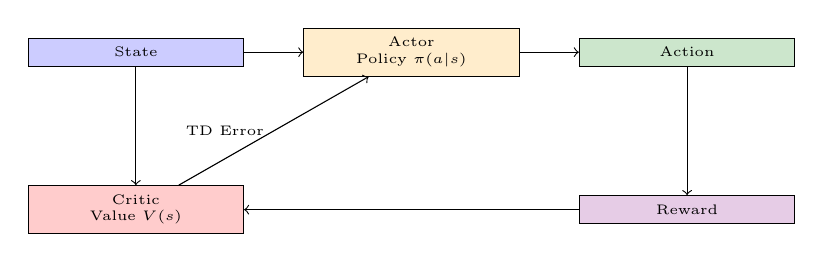
\begin{tikzpicture}[scale=0.5, every node/.style={font=\tiny}]
				\node[draw, rectangle, fill=blue!20, text width=2.5cm, align=center] (state) {State};
				\node[draw, rectangle, fill=orange!20, text width=2.5cm, align=center] (actor) [right of=state, xshift=2.5cm] {Actor\\Policy $\pi(a|s)$};
				\node[draw, rectangle, fill=green!20, text width=2.5cm, align=center] (action) [right of=actor, xshift=2.5cm] {Action};
				\node[draw, rectangle, fill=red!20, text width=2.5cm, align=center] (critic) [below of=state, yshift=-1cm] {Critic\\Value $V(s)$};
				\node[draw, rectangle, fill=purple!20, text width=2.5cm, align=center] (reward) [below of=action, yshift=-1cm] {Reward};
				\draw[->] (state) -- (actor);
				\draw[->] (state) -- (critic);
				\draw[->] (actor) -- (action);
				\draw[->] (action) -- (reward);
				\draw[->] (reward) -- (critic);
				\draw[->] (critic) -- (actor) node[midway,left] {TD Error};
			\end{tikzpicture}
		\end{center}
		
		\textbf{How It Works:}
		\begin{enumerate}
			\item Actor takes action based on current policy
			\item Critic evaluates the action (TD error)
			\item TD error: $\delta = R + \gamma V(s') - V(s)$
			\item If $\delta > 0$: Action was better than expected $\rightarrow$ increase probability
			\item If $\delta < 0$: Action was worse than expected $\rightarrow$ decrease probability
		\end{enumerate}
		
		\textbf{Advantages:}
		\begin{enumerate}
			\item \textcolor{green}{Lower variance} than policy gradient
			\item \textcolor{green}{Can learn online} (TD-based)
			\item \textcolor{green}{Continuous action spaces} (policy-based)
		\end{enumerate}
		
		\textcolor{red}{\textbf{Exam Trap:}} Actor-Critic combines \textcolor{blue}{policy} (actor) and \textcolor{blue}{value} (critic) learning!
	\end{frame}
	
	\begin{frame}{Policy Methods - Summary}
		\fontsize{6.5}{7.5}\selectfont
		\textcolor{blue}{\textbf{Policy Methods - Complete Summary}}
		
		\textbf{Key Concepts to Remember:}
		
		\begin{enumerate}
			\item \textcolor{blue}{Policy-Based Methods:}
			\begin{itemize}
				\item Learn policy $\pi_\theta(a|s)$ directly
				\item Output: action (or probability distribution)
				\item Better for continuous action spaces
			\end{itemize}
			
			\item \textcolor{blue}{Value-Based Methods:}
			\begin{itemize}
				\item Learn Q(s,a) or V(s)
				\item Output: value estimates
				\item Derive policy from values
				\item Better for discrete action spaces
			\end{itemize}
			
			\item \textcolor{blue}{REINFORCE:}
			\begin{itemize}
				\item MC policy gradient
				\item High variance
				\item Requires complete episodes
			\end{itemize}
			
			\item \textcolor{blue}{Actor-Critic:}
			\begin{itemize}
				\item Actor: Policy
				\item Critic: Value function
				\item Lower variance
				\item Can learn online
			\end{itemize}
			
			\item \textcolor{blue}{Advantages of Policy Methods:}
			\begin{itemize}
				\item Continuous actions
				\item Stochastic policies
				\item Better convergence
			\end{itemize}
			
			\item \textcolor{blue}{Disadvantages of Policy Methods:}
			\begin{itemize}
				\item Slow convergence
				\item Local optima
				\item Sample inefficient
			\end{itemize}
		\end{enumerate}
		
		\textcolor{red}{\textbf{Exam Success:}} Choose between value-based and policy-based based on \textcolor{blue}{action space} (discrete vs continuous)!
	\end{frame}
	
	% ============================================================
	% SECTION 6: MDP & BELLMAN - SLIDES 91-100
	% ============================================================
	
	\begin{frame}{MDP - Formal Definition}
		\fontsize{6.5}{7.5}\selectfont
		\textcolor{blue}{\textbf{Markov Decision Processes - The RL Framework}}
		
		\textbf{What is an MDP?}
		\begin{itemize}
			\item Mathematical framework for modeling decision-making
			\item Defined by: States, Actions, Transition Probabilities, Rewards
			\item Assumes the \textcolor{blue}{Markov property}
		\end{itemize}
		
		\textbf{MDP Components:}
		\begin{enumerate}
			\item \textcolor{blue}{States ($S$)}: Set of all possible states
			\item \textcolor{blue}{Actions ($A$)}: Set of all possible actions
			\item \textcolor{blue}{Transition Probability}: $P(s'|s,a)$
			\item \textcolor{blue}{Reward}: $R(s,a)$ or $R(s,a,s')$
			\item \textcolor{blue}{Discount Factor}: $\gamma \in [0,1]$
		\end{enumerate}
		
		\textbf{The Markov Property:}
		\[
		P(S_{t+1} | S_t, S_{t-1}, ..., S_1) = P(S_{t+1} | S_t)
		\]
		\begin{itemize}
			\item Future depends only on the \textcolor{blue}{current state}
			\item "Memoryless" property
			\item Simplifies analysis significantly
		\end{itemize}
		
		\textbf{Transition Probability Matrix:}
		\begin{itemize}
			\item $P$ = matrix where $P_{ij} = P(S_{t+1} = j | S_t = i)$
			\item For actions: $P^a_{ij} = P(S_{t+1} = j | S_t = i, A_t = a)$
			\item After $n$ steps: $P^n$ (matrix multiplication)
		\end{itemize}
		
		\textbf{Example - Simple 2-State MDP:}
		\begin{itemize}
			\item States: S1, S2
			\item Actions: Left, Right
			\item Transition: P(Left from S1 to S2) = 0.7, P(Left from S1 to S1) = 0.3
		\end{itemize}
		
		\textcolor{red}{\textbf{Exam Trap:}} MDPs assume the \textcolor{blue}{Markov property} - only the current state matters!
	\end{frame}
	
	\begin{frame}{Bellman Equations - Derivation}
		\fontsize{6.5}{7.5}\selectfont
		\textcolor{blue}{\textbf{Bellman Equations - The Recursive Foundation}}
		
		\textbf{The Bellman Equation (For a Fixed Policy):}
		\[
		V(s) = \sum_a \pi(a|s) \sum_{s'} P(s'|s,a) [R(s,a) + \gamma V(s')]
		\]
		
		\textbf{Derivation:}
		\begin{enumerate}
			\item $V(s) = E[G_t | S_t = s]$
			\item $G_t = R_{t+1} + \gamma G_{t+1}$
			\item $V(s) = E[R_{t+1} + \gamma V(S_{t+1}) | S_t = s]$
			\item Expand expectation over actions and next states
		\end{enumerate}
		
		\textbf{Bellman Optimality Equation:}
		\[
		V^*(s) = \max_a \sum_{s'} P(s'|s,a) [R(s,a) + \gamma V^*(s')]
		\]
		
		\textbf{For Q-Function:}
		\[
		Q(s,a) = \sum_{s'} P(s'|s,a) [R(s,a) + \gamma \max_{a'} Q(s',a')]
		\]
		
		\textbf{What They Tell Us:}
		\begin{itemize}
			\item Value of a state = immediate reward + discounted value of next state
			\item This is \textcolor{blue}{recursive}
			\item Can be solved using \textcolor{blue}{dynamic programming}
		\end{itemize}
		
		\textbf{Solving Bellman Equations:}
		\begin{itemize}
			\item If transition probabilities known: Dynamic Programming
			\item If not known: MC or TD methods
		\end{itemize}
		
		\textcolor{red}{\textbf{Exam Trap:}} Bellman equations are \textcolor{blue}{recursive} - they define V(s) in terms of V(s')!
	\end{frame}
	
	\begin{frame}{Bellman Equations - Examples}
		\fontsize{6.5}{7.5}\selectfont
		\textcolor{blue}{\textbf{Bellman Equations - Worked Examples}}
		
		\textbf{Example 1 - Simple MDP:}
		\begin{itemize}
			\item 2 states: S1, S2
			\item 2 actions: A1, A2 (deterministic)
			\item Rewards: R(S1,A1,S2) = 10, R(S2,A2,S1) = 5
			\item $\gamma = 0.9$
		\end{itemize}
		
		\textbf{Bellman Equations:}
		\begin{itemize}
			\item $V(S1) = 10 + \gamma V(S2)$
			\item $V(S2) = 5 + \gamma V(S1)$
		\end{itemize}
		
		\textbf{Solve:}
		\begin{itemize}
			\item $V(S1) = 10 + 0.9V(S2)$
			\item $V(S2) = 5 + 0.9V(S1)$
			\item Substitute: $V(S1) = 10 + 0.9(5 + 0.9V(S1)) = 10 + 4.5 + 0.81V(S1)$
			\item $0.19V(S1) = 14.5 \Rightarrow V(S1) = 76.32$
			\item $V(S2) = 5 + 0.9(76.32) = 73.69$
		\end{itemize}
		
		\textbf{Example 2 - Grid World:}
		\begin{itemize}
			\item Agent in 3x3 grid
			\item Goal: Reach top-right corner
			\item Reward: +1 at goal, -1 for walls
			\item $\gamma = 0.9$
		\end{itemize}
		
		\textbf{Bellman Optimality:}
		\[
		V^*(s) = \max_a \sum_{s'} P(s'|s,a)[R(s,a) + \gamma V^*(s')]
		\]
		\begin{itemize}
			\item Solve iteratively (value iteration)
			\item Converges to optimal values
		\end{itemize}
		
		\textcolor{red}{\textbf{Exam Trap:}} Bellman equations can be \textcolor{blue}{solved analytically} for simple MDPs!
	\end{frame}
	
	\begin{frame}{RL - Complete Summary}
		\fontsize{6.5}{7.5}\selectfont
		\textcolor{blue}{\textbf{Reinforcement Learning - Complete Summary}}
		
		\textbf{Core Concepts:}
		\begin{itemize}
			\item Agent learns through \textcolor{blue}{trial and error}
			\item Goal: \textcolor{blue}{Maximize cumulative reward}
			\item Policy: Strategy for choosing actions
			\item Value functions: V(s) and Q(s,a)
		\end{itemize}
		
		\textbf{The Three Strategies (MAB):}
		\begin{enumerate}
			\item Greedy (Pure Exploitation)
			\item Random (Pure Exploration)
			\item $\epsilon$-Greedy (Balanced) - \textcolor{green}{Best practical choice}
		\end{enumerate}
		
		\textbf{Two Main Approaches:}
		\begin{enumerate}
			\item \textcolor{blue}{Monte Carlo (MC):}
			\begin{itemize}
				\item Episode-end updates
				\item Uses actual returns $G_t$
				\item Unbiased, high variance
				\item Episodic tasks only
			\end{itemize}
			\item \textcolor{blue}{Temporal Difference (TD):}
			\begin{itemize}
				\item Step-by-step updates
				\item Uses bootstrapping
				\item Biased, low variance
				\item Episodic and continuous tasks
			\end{itemize}
		\end{enumerate}
		
		\textbf{Two Families of Algorithms:}
		\begin{enumerate}
			\item \textcolor{blue}{Value-Based:}
			\begin{itemize}
				\item Q-learning (off-policy)
				\item SARSA (on-policy)
				\item DQN (deep learning)
			\end{itemize}
			\item \textcolor{blue}{Policy-Based:}
			\begin{itemize}
				\item REINFORCE (MC)
				\item Actor-Critic
				\item Policy Gradient
			\end{itemize}
		\end{enumerate}
		
		\textcolor{red}{\textbf{Exam Success:}} Master the \textcolor{blue}{exploration-exploitation} trade-off - it's the heart of RL!
	\end{frame}
	
	\begin{frame}{FINAL EXAM TIPS - RL}
		\fontsize{6.5}{7.5}\selectfont
		\textcolor{blue}{\textbf{Top 15 RL Exam Traps to Remember:}}
		
		\begin{enumerate}
			\item \textcolor{red}{Trap 1:} RL output is a \textcolor{blue}{policy} (strategy), not a prediction or classification
			\item \textcolor{red}{Trap 2:} MAB has \textcolor{blue}{ONLY ONE state} - actions don't change the environment
			\item \textcolor{red}{Trap 3:} $\epsilon$-greedy: random number $<$ $\epsilon$ $\rightarrow$ \textcolor{blue}{explore}; $\ge$ $\rightarrow$ \textcolor{blue}{exploit}
			\item \textcolor{red}{Trap 4:} $\epsilon$ decays as $\epsilon_t = \beta^{t-1}$ (not $\beta^t$)
			\item \textcolor{red}{Trap 5:} MC updates \textcolor{blue}{at episode end} using $G_t$; TD updates \textcolor{blue}{every step} using $R_{t+1} + \gamma V(s')$
			\item \textcolor{red}{Trap 6:} MC = \textcolor{blue}{unbiased but high variance}; TD = \textcolor{blue}{biased but low variance}
			\item \textcolor{red}{Trap 7:} Q-learning is \textcolor{blue}{off-policy}; SARSA is \textcolor{blue}{on-policy}
			\item \textcolor{red}{Trap 8:} $\alpha$ = \textcolor{blue}{learning rate}; $\gamma$ = \textcolor{blue}{discount factor}; $\epsilon$ = \textcolor{blue}{exploration rate}
			\item \textcolor{red}{Trap 9:} DQN uses \textcolor{blue}{experience replay} + \textcolor{blue}{target network} for stability
			\item \textcolor{red}{Trap 10:} Policy-based methods handle \textcolor{blue}{continuous action spaces}; value-based methods handle discrete actions
			\item \textcolor{red}{Trap 11:} MC requires \textcolor{blue}{episodic tasks} (terminal states); TD handles continuous tasks
			\item \textcolor{red}{Trap 12:} Bellman equations are \textcolor{blue}{recursive} - V(s) depends on V(s')
			\item \textcolor{red}{Trap 13:} MDPs assume the \textcolor{blue}{Markov property} - only the current state matters
			\item \textcolor{red}{Trap 14:} Actor-Critic = \textcolor{blue}{Actor} (policy) + \textcolor{blue}{Critic} (value)
			\item \textcolor{red}{Trap 15:} RLHF is \textcolor{blue}{RL from human feedback} - used for fine-tuning LLMs
		\end{enumerate}
		
		\textcolor{blue}{\textbf{Remember:}} RL is about \textcolor{blue}{learning optimal behavior through experience}! The exam tests conceptual understanding of the trade-offs between methods.
	\end{frame}
	
\end{document}